\documentclass[a4paper]{article}

% CJK support: prefer ctex, fallback to XeTeX native line breaking
\IfFileExists{ctex.sty}{
  \usepackage[fontset=fandol]{ctex}
}{
  % Fallback for minimal TeX installs (e.g. MacTeX Basic, TeX Live scheme-basic)
  % without ctex/xeCJK. Uses XeTeX's built-in CJK line breaking.
  \usepackage{fontspec}
  \XeTeXlinebreaklocale "zh"
  \XeTeXlinebreakskip = 0pt plus 1pt
  \IfFontExistsTF{Songti SC}{\setmainfont{Songti SC}}{%
    \IfFontExistsTF{Noto Serif CJK SC}{\setmainfont{Noto Serif CJK SC}}{}%
  }
  \IfFontExistsTF{Heiti SC}{\setsansfont{Heiti SC}}{%
    \IfFontExistsTF{Noto Sans CJK SC}{\setsansfont{Noto Sans CJK SC}}{}%
  }
}

% Basic packages
\usepackage{amsmath, amssymb}
\usepackage{graphicx}
\usepackage[margin=2.5cm]{geometry}
\usepackage[most]{tcolorbox}
\usepackage{etoolbox}
\usepackage{listings}
\usepackage{hyperref}
\usepackage{booktabs}
\usepackage{subcaption}
\usepackage{float}
\usepackage{tikz}
\IfFileExists{pgfplots.sty}{
    \usepackage{pgfplots}
    \pgfplotsset{compat=1.18}
}{}

% ===== Highlight boxes =====
\newtcolorbox{knowledgebox}[1]{
    enhanced, colback=blue!5!white, colframe=blue!75!black, colbacktitle=blue!75!black,
    coltitle=white, fonttitle=\bfseries, title=#1, attach boxed title to top left={yshift=-2mm, xshift=2mm},
    boxrule=1pt, sharp corners
}

\newtcolorbox{importantbox}[1]{
    enhanced, colback=yellow!10!white, colframe=yellow!80!black, colbacktitle=yellow!80!black,
    coltitle=black, fonttitle=\bfseries, title=#1, sharp corners
}

\newtcolorbox{warningbox}[1]{
    enhanced, colback=red!5!white, colframe=red!75!black, colbacktitle=red!75!black,
    coltitle=white, fonttitle=\bfseries, title=#1, sharp corners
}

% ===== Code listings =====
\lstset{
    basicstyle=\ttfamily\small,
    keywordstyle=\color{blue},
    stringstyle=\color{red!60!black},
    commentstyle=\color{green!60!black},
    breaklines=true,
    frame=single,
    numbers=left,
    numberstyle=\tiny\color{gray},
    captionpos=b,
    extendedchars=false
}

% ===== Figure provenance and unit macros =====
% \vtag goes inside \caption{...}; \srcnote{MM:SS--MM:SS} follows the figure environment.
\newcommand{\vtag}{\protect\footnotemark}
\newcommand{\srcnote}[1]{\footnotetext{视频画面时间区间：#1。若为裁剪图，时间区间仍对应原视频画面。}}
% Units work in text and math mode; never hand-write $^\circ$ or \AA inside \mathrm.
\newcommand{\degC}{\ensuremath{^{\circ}\mathrm{C}}}
\newcommand{\um}{\ensuremath{\mu\mathrm{m}}}
\newcommand{\nm}{\ensuremath{\mathrm{nm}}}
\newcommand{\angstrom}{\ensuremath{\text{\AA}}}

% ===== Front-page metadata =====
% Fill these in when generating notes.
\newcommand{\notetitle}{需求和架构（一）：当代码变便宜之后}
\newcommand{\notesubtitle}{从教务系统的需求泥潭到汉诺塔、二维码与 Event Sourcing —— 南京大学《生成式软件工程》第 6 讲}
\newcommand{\noteauthors}{lecture-to-notes}
\newcommand{\notedate}{\today}
\newcommand{\videochannel}{绿导师原谅你了（蒋炎岩）}
\newcommand{\videopublishdate}{2026-09-22}
\newcommand{\videoduration}{约 97 分钟}
\newcommand{\videourl}{https://www.bilibili.com/video/BV1Rch76WEfQ/}
\newcommand{\videocoverpath}{cover.jpg}

\begin{document}

% ===== Title page =====
\begin{titlepage}
\centering
{\Large 课程笔记\par}
\vspace{1.2cm}
{\huge\bfseries \notetitle\par}
\ifdefempty{\notesubtitle}{}{
\vspace{0.3cm}
{\large \notesubtitle\par}
}
\vspace{0.5cm}
{\large \noteauthors\par}
\vspace{0.3cm}
{\large \notedate\par}
\vspace{1.0cm}

\ifdefempty{\videocoverpath}{
{\small 请在生成笔记时填入视频封面图的本地路径。\par}
}{
\includegraphics[width=0.82\textwidth,height=0.40\textheight,keepaspectratio]{\videocoverpath}\par
}

\vfill
\begin{tcolorbox}[width=0.9\textwidth, colback=black!2!white, colframe=black!60, sharp corners]
\textbf{视频作者/频道}：\videochannel\par
\textbf{发布日期}：\videopublishdate\par
\textbf{视频时长}：\videoduration\par
\textbf{视频链接}：
\ifdefempty{\videourl}{
未填写
}{
\href{\videourl}{\nolinkurl{\videourl}}
}
\end{tcolorbox}
\end{titlepage}

\tableofcontents
\newpage

%% --- 正文内容开始 --- %%
\section*{导读}

这一讲回答一个问题：当 AI 已经能廉价地写出“目标明确”的代码，软件工程里还剩下什么难题？讲者蒋炎岩的回答是需求、产品设计和架构。需求决定软件往哪个方向走，架构决定软件在需求不断变化时还能走多远；两者一旦做错，AI 生成代码的速度只会让错误更快地堆成“屎山”。

全讲沿着三个问题展开。第一，需求为什么这么难：讲者现场打开南京大学的教务系统，又让 GPT 先调研它、写出一份需求说明书、再照着说明书实现一个演示系统，用这个身边的例子说明需求会爆炸、说不清、还会变。第二，架构到底是什么：讲者从 10 行的非递归汉诺塔、2000 行的 Excel 二维码生成器一路讲到 50 万行的教务系统，反复使用同一条方法——“跳出问题看问题”。第三，教务系统这类业务系统该用什么架构：讲者指出常见的 CRUD（增删改查）架构只保存“当前状态”，会把历史事实、规则和决定混在一起；把事件历史当作一等公民的 Event Sourcing，是从第一性原理推出来的更好选择。

本讲义按这三个问题重排了课堂内容，课堂上的即兴演示（包括一次电脑死机的诊断）只在它们支撑论点时保留。文中“讲者认为”标出的是讲者的判断；“本讲义整理为”标出的是笔记作者的归纳。

\section{回顾：从意图到实现，软件为什么“不软”}

本节回答：上一讲留下的 Intent–Spec–Impl 框架是什么，为什么需求和架构这一段最难用传统方法研究？

\subsection{从意图到实现：瀑布与数据依赖图}

上一讲从软件危机讲到软件工程的起源。讲者用板书把 Royce 那篇老论文里的理想流程画成三层：先有意图（intent），意图进入规格说明（specification），规格再落到实现（implementation），实现之后还要维护，软件的生命周期并没有结束。一路向下，自然就是“瀑布”的形状。

这三层之间是一张错综复杂的依赖网络。需求阶段形成的认识进入规格，规格之间彼此依赖；实现阶段又有模块、函数、代码、测试等各种制品（artifact），它们与上游之间有直接和间接的数据依赖（data dependency）。Royce 对瀑布模型的批判正来自这张图：如果在下游发现一个错误，而它回溯到上游某个需求或设计本身就是错的，那么被它“污染”的整片下游都会失效，需要重做，成本巨大。软件工程研究的就是在需求分析、系统设计、系统实现各个阶段用什么方法降低这种代价——既包括写测试、做自动化分析这类技术方法，也包括产品经理如何管人、如何用 checklist 这类带有人文关怀的方法。

\begin{figure}[H]
\centering
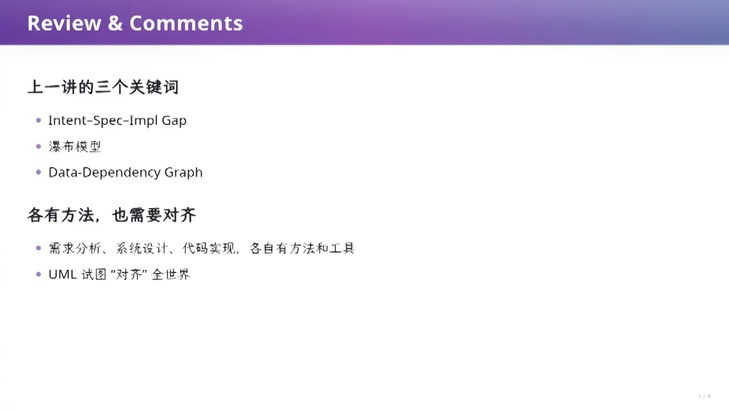
\includegraphics[width=\textwidth]{figures/fig_01_review_keywords.jpg}
\caption{上一讲的三个关键词：Intent–Spec–Impl Gap、瀑布模型、数据依赖图；需求分析、系统设计、代码实现各有方法和工具，UML 试图“对齐”全世界\vtag}
\end{figure}
\srcnote{00:00:30--00:00:44}

\begin{knowledgebox}{背景：可追溯性（traceability）与 UML}
在 AI 之前，人和人很难对齐；如果不写文档、只剩一份代码，出了错甚至不知道该追溯到过去的哪个决定。软件工程因此提出了可追溯性：理想情况下，每一个测试用例、每一段代码都能关联到过去的某个需求或设计。这样“改它会影响谁、改设计会影响哪些测试”都能被维护起来。若再有一种结构化、有语义的语言来表示这张关系图就更好，于是有了 UML，它试图统一全世界的软件工程实践。讲者肯定这些方法“都是有智慧的”，后文的需求说明书案例会展示编号 ID 如何承担可追溯性的职能。
\end{knowledgebox}

\subsection{软件不软：纯逻辑制品容不下细微差错}

讲者接着指出软件工程困难的一个本质原因：软件并不“软”。教室里的椅背是软的，你一靠它就扁下去，站起来又弹回原样，下次坐还是好的。软件是纯粹的逻辑制品，有形式语义，容不下任何细微的差错。

讲者举了一个极端例子：程序从标准输入读一个 $N$，然后循环读 $N$ 个数到数组里。若程序运行在卫星上，一束宇宙射线击中内存，把 $N=1$ 这个无符号整数的最高位翻成 1，$N$ 就变成一个巨大的数，程序会无限制地读输入——没有输入时表现为卡死，读了一两千个数之后可能内存出错。这不只是太空里的事：讲者提到数据中心里也能观察到，随着处理器制程越来越先进，某些高密度指令会产生 silent error，同一条指令在这台机器和那台机器上结果不同，而且可能要服务运行一段时间之后才暴露出这种制造缺陷。

\begin{figure}[H]
\centering
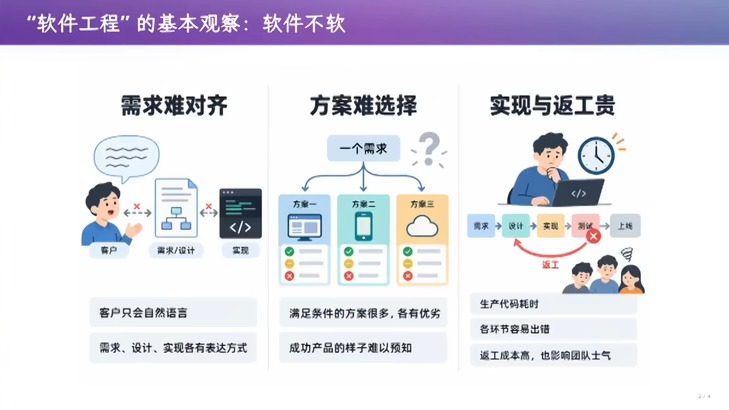
\includegraphics[width=\textwidth]{figures/fig_02_software_not_soft.jpg}
\caption{“软件工程”的基本观察：软件不软。三个困难分别是需求难对齐（客户只会自然语言，需求、设计、实现各有表达方式）、方案难选择（满足条件的方案很多且各有优劣，成功产品的样子难以预知）、实现与返工贵（生产代码耗时，各环节容易出错，返工成本高且影响团队士气）\vtag}
\end{figure}
\srcnote{00:03:30--00:03:44}

图中的三个困难与上一小节的依赖图是一回事的两面：需求难对齐，意味着依赖图的上游本身就可能是错的；方案难选择，意味着同一个需求可以长出很多棵不同的下游子树；实现与返工贵，意味着上游一旦改变，下游的代价要真金白银地付出。

\subsection{为什么需求、产品、架构这么难研究}

讲者观察到，软件工程学界的研究大部分集中在编码和实现附近，因为需求、产品、架构太难定量研究了。他半开玩笑地说，学校里的“软工人”都不在做“软工”，反而去研究“缺陷预测”这类领域；有些做自然语言处理的研究者会说，traceability 很重要，那就训练一个神经网络从数据里推导它。

\begin{figure}[H]
\centering

\includegraphics[width=\textwidth]{figures/fig_03_wicked_problems.jpg}
\caption{软件工程方法与研究：需求、产品、架构都太难定量研究；一个来自城市规划的参照——难的不只是“怎么测”，不同参与者可能连“什么算成功”都没有共识，参见 Wicked Problems（Rittel \& Webber, 1973）\vtag}
\end{figure}
\srcnote{00:08:15--00:08:29}

\begin{knowledgebox}{背景：Wicked Problems}
幻灯片引用的 Rittel 和 Webber 1973 年的论文来自城市规划领域。这类问题的特征是：问题怎样定义，本身就取决于各方的利益与价值判断，因此没有一个大家公认的“成功”标准可供测量。后文的“教务系统需求泥潭”会再次引用它：学生要选上课、教师要控制班额、教务员要保证毕业，冲突由谁裁决，是技术之外的问题。
\end{knowledgebox}

讲者还解释了计算机专业的课程为什么“从底下开始学”：软件工程关乎整个软件生命周期，但如果没有亲手写过代码、没有体会过开发的痛苦，就不可能判断一个设想“能不能办到、要花多少成本”，也就做不好产品经理。所以学生先学一门基础的编程语言，在这个基础上不断产生新的知识，知道世界是怎么失败的、新的语言为什么被创造出来，再一点一点往上走。本讲讨论的需求、产品、架构，正处在从 intent 到 spec 的阶段；课程前面先讲版本管理，是因为任何软件都从一个空仓库出发，接下来就要把控软件往哪个方向开。

\subsection{本章小结}

软件工程的起点是一张从意图到实现的依赖图：上游的错误会沿着依赖污染整片下游，而软件作为纯逻辑制品又没有“弹性”去吸收这些错误。可追溯性、UML 等方法试图把这张图管理起来，但需求、产品和架构这一段恰恰最难定量研究。下一节要问的是：AI 把写代码的成本压低之后，这一段的地位发生了什么变化。

\section{AI 时代：为什么需求、产品和架构成了杠杆}

本节回答：既然 AI 能便宜地写代码，为什么讲者说需求、产品设计和架构反而成了撬动软件生产力的杠杆？

\subsection{目标明确的代码已经极为便宜}

讲者的判断是：在 AI 时代，生产一段目标明确的代码已经非常便宜。他自述现在让 AI 生成代码时，只要把边界划清楚，已经真的不看它的实现；他后面展示的 GPT-6 汉诺塔代码“已经超越人类能够理解的范畴”，但它是对的，他也比较信任它。只要边界清楚，并且知道怎样做好维护，就可以把 Agent Swarm（成群并行工作的智能体）铺开，实现有一定质量保证的软件。幻灯片还列出 Agent 也能写测试用例、断言，甚至证明。

\begin{figure}[H]
\centering
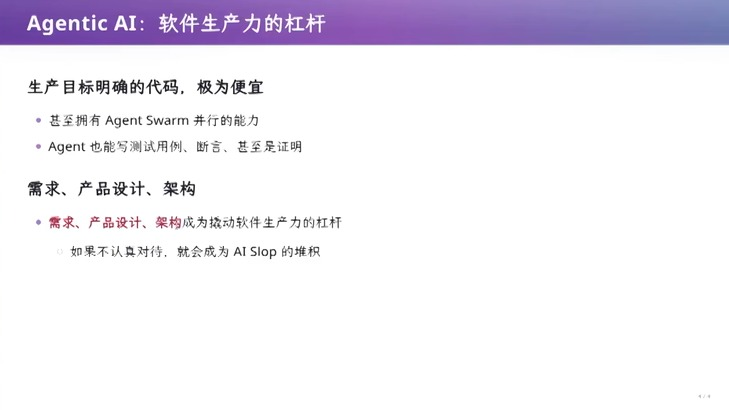
\includegraphics[width=\textwidth]{figures/fig_04_agentic_leverage.jpg}\\[4pt]
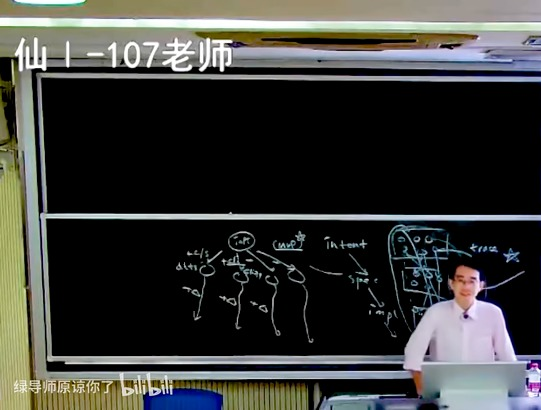
\includegraphics[width=0.72\textwidth]{figures/fig_04_board_intent_spec_mvp.jpg}
\caption{上：Agentic AI 让“生产目标明确的代码”极为便宜，需求、产品设计、架构成为撬动软件生产力的杠杆，如果不认真对待就会成为 AI Slop 的堆积。下：同一时刻的板书，右侧是 intent→spec→impl 的依赖与 trace，左侧是从同一个 MVP 需求出发、因提示词不同（如 CLI、client–server）而分叉出的几条实现路径\vtag}
\end{figure}
\srcnote{00:13:45--00:13:59}

于是剩下的压力集中到一处：什么东西决定一个软件系统最后能走多远。讲者认为，这就是需求、产品设计和架构。

\subsection{MVP 的本能：不做即将扔掉的东西}

做软件的人都熟悉 MVP（minimum viable product，最小可行产品）。讲者认为做 MVP 本身没有问题，它能让你快速找到一条从 intent 到 specification 再到 implementation 的路径，在这条路径上走完软件的完整流程，只是它不完备。

做 MVP 时人们会本能地先做最重要的功能，不会先去调按钮的样式。讲者用依赖图解释这个本能：按钮样式依赖整个界面设计，界面设计又依赖所有功能的实现；上游还不确定时去打磨下游，一旦上游变化，按钮样式很可能就不合适了。每个人都有“不做无用功、不研究即将扔掉的东西”的本能，按这个本能选最重要的功能，就会得到一个能运行的版本。

\subsection{几个字的提示词，会长成不同的软件}

问题在于 AI。讲者指出，至少今天的 AI 不会主动从需求、产品设计和架构的角度思考，除非你用 prompt 显式地告诉它。而哪怕只是几个字的提示，也会让同一个 MVP 需求长出完全不同的软件：要求做成命令行（CLI）架构，项目里可能就出现一个 \texttt{cli.py}，或依赖 Claude Code 所用的那类 JavaScript 命令行库；要求 client–server 架构，它可能先设计数据存储、选一个数据库，写出一个 \texttt{db.ts}。这些 MVP 功能上看起来差不多，都实现了“做一个 coding agent”或“做一个 Lab 1 的随身 agent”之类的需求。

这些文件一旦写出来，就进入了 Agent 的上下文；此后每做一个新需求，都会带上之前全部的历史。软件工程里有个名词叫技术债（technical debt）：你做任何决定，都背上了这个决定的债务，而在做 MVP 的时候，你并不知道这个决定是好是坏。

\begin{importantbox}{讲者的论点：三根杠杆}
决定会从哪里来？来自需求（你到底要什么功能——想做辅助学习的工具，还是已进科研组、对读论文有强烈需求）、来自产品设计（只给自己用的软件可以很顺手，给别人用时，你自己的知识和偏好可能让对方不习惯），以及一个隐藏因素——架构，即这个软件将来会变成什么样。讲者认为这三者是撬动软件生产的真正杠杆：在 AI 生成代码的过程中，它们对技术债的累积有极大影响。因此本讲和下一讲都讲需求和架构。
\end{importantbox}

\begin{warningbox}{AI 默认不会偿还的技术债：日志}
课上讲者的电脑发生了一次故障：系统界面和 OBS 推流还在工作，但鼠标、键盘全部失灵，插上新鼠标也没用。讲者让 Agent 读系统日志诊断（终端里显示的是 \texttt{journalctl} 与 USB/xHCI 控制器相关的内核日志，Agent 给出了把设备换到另一条 USB 控制器、复现时观察 \texttt{dmesg} 等建议）。讲者借此指出一条工程实践：出了问题要看日志，这要求写软件时就输出足够多的日志。如果你不要求，AI 也不会主动做，它会生成一个没有任何日志的系统——这同样是在留下技术债。
\end{warningbox}

\subsection{本章小结}

代码生成变便宜之后，稀缺的是“往哪走”和“走多远”的判断。MVP 的本能在人类开发中有效，但交给 AI 时，几个字的提示就会把软件推向不同的依赖结构，并随着上下文一路累积成技术债。要在 AI 时代控制这种累积，就得认真对待需求、产品设计和架构。下一节先看需求：为什么它过去难教，而现在可以用 AI 直接演示。
\section{需求工程：用 AI 把教务系统“做一遍”}

本节回答：需求工程过去为什么难教，一份像样的需求说明书长什么样，以及当需求写清楚之后 AI 能替你做到哪一步？

\subsection{需求工程曾经很难讲}

讲者说，需求工程过去很难讲，因为学生不会去见真正的客户，也做不了“需求”级别的软件系统。从学第一门编程语言到毕业，学生的能力增长通常不足以面对一个真实的软件客户。

\begin{figure}[H]
\centering
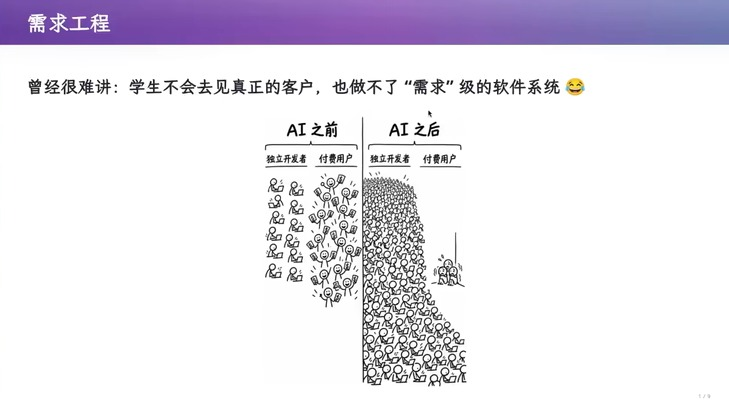
\includegraphics[width=\textwidth]{figures/fig_05_req_eng_before_after.jpg}
\caption{需求工程曾经很难讲：学生不会去见真正的客户，也做不了“需求”级的软件系统。漫画对比 AI 之前与 AI 之后的独立开发者与付费用户数量\vtag}
\end{figure}
\srcnote{00:15:00--00:15:14}

这件事正在变化。讲者描述漫画：AI 之前，只有少量经过多年开源社区洗礼的精英独立开发者，服务一些付费用户；AI 之后，独立开发者数量爆炸，付费用户反倒“瑟瑟发抖”。换句话说，今天一个学生借助 AI 已经可以做出需求级的系统，需求工程终于可以用真实案例来讲。

\subsection{现场观察：教务系统的“史诗级需求爆炸”}

讲者选的案例是南京大学的教务系统。他现场扫码登录，展示了一个新近出现的 AI 搜索功能：问“仙林教学楼的灯一直没有解决，我应该打电话给谁”，系统给出基础设施部的联系电话与职责范围；问“我现在在上什么课”，系统也能返回教师课表。讲者说这显然是一次“史诗级更新”，而此前他在平台上报修，基建处回复“这个事情不归我们管”。

\begin{figure}[H]
\centering

\includegraphics[width=\textwidth]{figures/fig_06_jw_ai_search.jpg}
\caption{教务系统网上办事大厅中的 AI 搜索：询问仙林教学楼照明维修，系统回复应联系基础设施部，并列出联系电话、部门名称和职责范围\vtag}
\end{figure}
\srcnote{00:17:00--00:17:14}

接着讲者点开“我的教学任务”等页面，一路展示这个系统里“无穷多的功能”：编辑联系方式、当前教学学期、最新排课学期、历史授课信息、期末考试签到表（考试安排发布前点击会弹窗提示无法打印）、编辑教材（当场点出一个 bug）、查看大纲、教学周历、助教管理等。他特别指出需求是不断叠加的：疫情之前没有慕课功能；疫情时领导要求为老师添加慕课，添加之后又要慕课助教，而且慕课助教不能当成普通教学班的助教，于是系统里多了一套新的页面和规则；新增、删除操作还要受“可维护时段”限制。

讲者的评价有两面。一面是讽刺：这样的系统肯定花了很多钱，某种程度上还不如把钱变成 token 补贴给大家——用 Agent 去查一次信息可能只要一两毛钱。另一面是承认：它确实做了需求分析，页面上的学期选择框、按考试安排控制的打印按钮，都是认真对齐过用户需求的痕迹。

\subsection{用魔法打败魔法：让 GPT 写一份需求说明书}

回到“学生见不到客户”的问题。讲者说，学生也不敢拍胸脯说“给我 20 万，我找几个同学把南大的教务系统包了”：签了合同，交付时达不到功能要求或非功能要求怎么办？学生不敢，“Agent 敢就行”。他让 GPT-6 Astra 先去调研教务系统的需求，再直接实现一个；幻灯片写着“一个 \texttt{/goal}，一小时完成任务”。调研只针对教师相关的功能，产出是一份需求说明书。

\begin{figure}[H]
\centering

\includegraphics[width=\textwidth]{figures/fig_07_srs_cover.jpg}
\caption{GPT 生成的《南京大学本科教学服务平台需求说明书》（教师视角·软件工程课程案例）：版本 1.0 为调研与候选需求基线，编制依据是当前教师账号在网上办事大厅中的实际页面观察\vtag}
\end{figure}
\srcnote{00:24:00--00:24:14}

封面页写明了这份文档的边界：它回答“一个本科教师如何在学期前、授课中、考核后和学生指导过程中完成教学事务，以及系统应提供怎样的功能、信息、约束和反馈”；它要把现有页面重构为“可讨论、可追溯、可验收”的需求，而不是菜单说明书或数据库设计；它是课堂案例研究版的需求基线，不代表校方批准的正式需求，也没有做真实的业务提交、成绩修改、审核决定或打印导出验证。

\begin{figure}[H]
\centering
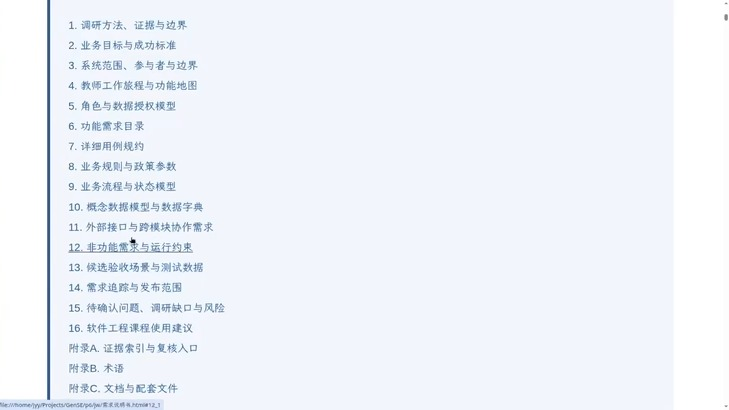
\includegraphics[width=\textwidth]{figures/fig_08_srs_toc.jpg}
\caption{需求说明书目录：从调研方法、证据与边界，业务目标与成功标准，到功能需求目录、非功能需求、候选验收场景、需求追踪与发布范围，最后是证据索引、术语、文档与配套文件等附录\vtag}
\end{figure}
\srcnote{00:24:30--00:24:44}

讲者对目录的解读是：GPT 懂软件工程。在我们看来教务系统已经做好了，突然写出这么多东西像是 slop；但如果你面对的是真正的客户，这些章节都有用处。例如术语表：客户看不懂某个词时可以去查，查完就对齐了。它们还处在早期的意图沟通阶段，并不是 UML 那样的形式化模型，但显然有一定用处。

\begin{figure}[H]
\centering
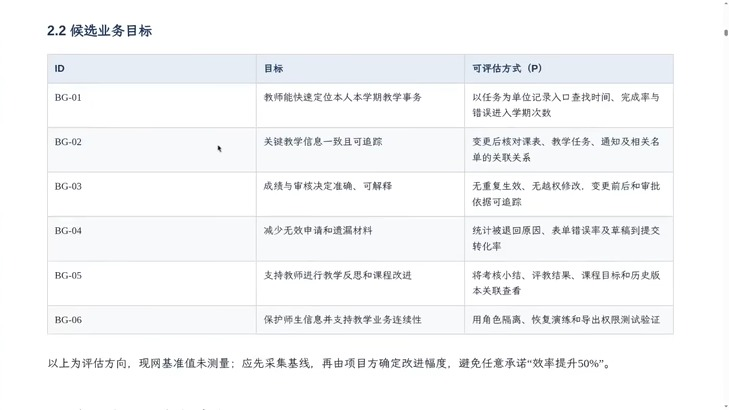
\includegraphics[width=\textwidth]{figures/fig_09_business_goals.jpg}
\caption{2.2 候选业务目标：BG-01 至 BG-06，每条目标配有“可评估方式”；表下注明这些只是评估方向，现网基准值未测量，应先采集基线，避免任意承诺“效率提升 50\%”\vtag}
\end{figure}
\srcnote{00:25:30--00:25:44}

\begin{figure}[H]
\centering
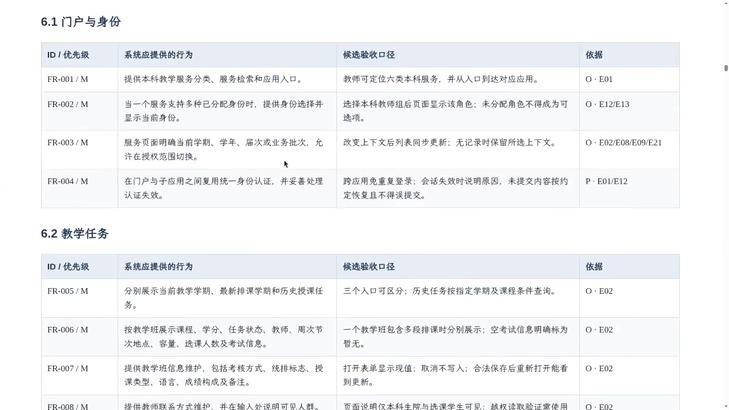
\includegraphics[width=\textwidth]{figures/fig_10_functional_reqs.jpg}
\caption{6.1 门户与身份、6.2 教学任务：每条功能需求都有 ID 与优先级（如 FR-001 / M）、系统应提供的行为、候选验收口径，以及依据（O 表示来自观察，P 表示拟议，E 为证据编号）\vtag}
\end{figure}
\srcnote{00:26:45--00:26:59}

下表 摘录了图中“门户与身份”的四条需求。讲者提醒，真正做软件时复杂性就在这些条目里：某个页面上“有还是没有”身份选择框，不写下来就永远说不清。

\begin{table}[H]
\centering
\small
\begin{tabular}{p{1.6cm}p{4.8cm}p{5.0cm}p{2.8cm}}
\toprule
ID/优先级 & 系统应提供的行为 & 候选验收口径 & 依据 \\
\midrule
FR-001 / M & 提供本科教学服务分类、服务检索和应用入口 & 教师可定位六类本科服务，并从入口到达对应应用 & O·E01 \\
FR-002 / M & 一个服务支持多种已分配身份时，提供身份选择并显示当前身份 & 选择本科教师组后页面显示该角色；未分配角色不得成为可选项 & O·E12/E13 \\
FR-003 / M & 页面明确当前学期、学年、届次或业务批次，允许在授权范围内切换 & 改变上下文后列表同步更新；无记录时保留所选上下文 & O·E02/E08/ E09/E21 \\
FR-004 / M & 门户与子应用之间复用统一身份认证，并妥善处理认证失效 & 跨应用免重复登录；会话失效时说明原因，未提交内容按约定恢复且不得误提交 & P·E01/E12 \\
\bottomrule
\end{tabular}
\caption{需求说明书“6.1 门户与身份”摘录（据 00:26:45 画面整理）}
\label{tab:fr}
\end{table}

\begin{importantbox}{编号 ID 如何提供可追溯性}
讲者强调，这份文档“是有 traceability 的”：每一个需求点前面都有角色、参与者或业务目标，而且每一条都有带形式语义的编号。自然语言里人人都会说“教学班和学生管理有关”，但只有 FR-002、BG-02、E12 这样的 ID 能把一条需求、它服务的业务目标和支撑它的证据确定地连起来，从而在一定程度上替你做了可追溯性。第 1 节提到的 UML 想做的是同一件事。
\end{importantbox}

\subsection{需求清单、追踪矩阵与验收场景：管理者的抓手}

除了 HTML 版说明书，GPT 还交付了几份结构化文件。

\begin{figure}[H]
\centering
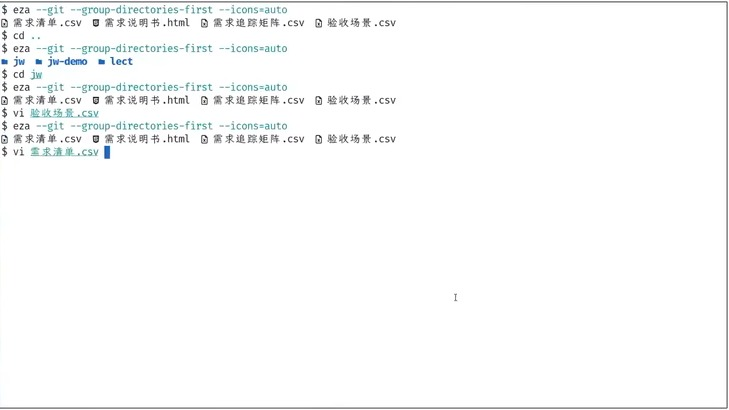
\includegraphics[width=\textwidth]{figures/fig_11_srs_artifacts.jpg}
\caption{需求交付物目录：需求清单.csv、需求说明书.html、需求追踪矩阵.csv、验收场景.csv\vtag}
\end{figure}
\srcnote{00:29:30--00:29:44}

讲者解释了这些文件“为了挣钱”的用途：验收场景定义了交付时怎样算完成；结构化的需求清单是一个 checklist，可以把前 20 个需求分给一个团队、后 20 个分给另一个团队，然后追踪每个人的进度，知道哪个团队的实现落后了。有了可追溯性，管理者就能把团队管起来。讲者也坦言，这部分内容本科课堂通常不怎么学。

\begin{knowledgebox}{学生第一次见到的长需求文档}
讲者认为，大作业做到一定规模，训练是相通的。在此之前，OJ 题目是很短的需求文档：输入输出接口明确而简单，一般就是读几个空格分隔的整数。学生第一次见到较长的 specification，是在计算机系统基础课实现全系统模拟器 NEMU 的时候：第一个实验要实现一个调试器，第二个实验要实现指令解释——“实现指令”只是一句话，但指令的行为写在手册里，于是得到了一份更大的需求文档。讲者据此说，学计算机系统基础时，某种程度上也在学软件工程。
\end{knowledgebox}

\subsection{AI 的魅力时刻：只凭说明书实现一个教务系统}

讲者又做了一件事：让 GPT 起一个 subagent（子智能体），不看任何现有教务系统，只根据这份需求说明书实现一个假的教务系统。得到的演示系统（界面名为“南雍教学”）可以浏览本周教学安排、编辑教材选用记录、查看学生名单、记录缺课。讲者的感受是“突然你又有信心了”：好像 20 万的合同也可以谈一谈了。

\begin{figure}[H]
\centering
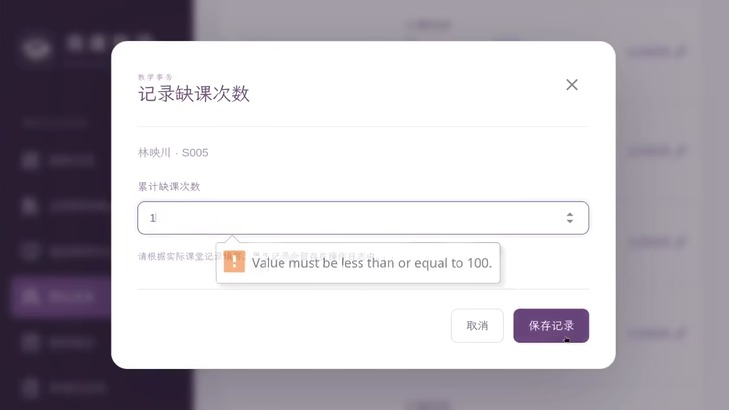
\includegraphics[width=\textwidth]{figures/fig_12_absence_validation.jpg}
\caption{subagent 仅凭需求说明书实现的演示系统：记录缺课次数时，前端校验拒绝过大的数值（提示“Value must be less than or equal to 100”）\vtag}
\end{figure}
\srcnote{00:31:45--00:31:59}

演示里也能看到它的局限与偏好：学生名单里的名字是 GPT 起的，风格“挺文雅”；缺课次数不允许输入负数，输入过大的数会被拒绝，但讲者指出，它仍允许记录一个超过全部上课次数总和的数，这也不合理。讲者由此给出的判断是：当需求文档写到这个程度时，编码、可追溯性、测试这些事情 AI 都能帮你搞定，“你只需要一份需求就行了”。

\subsection{需求就是和客户无尽地沟通}

\begin{figure}[H]
\centering
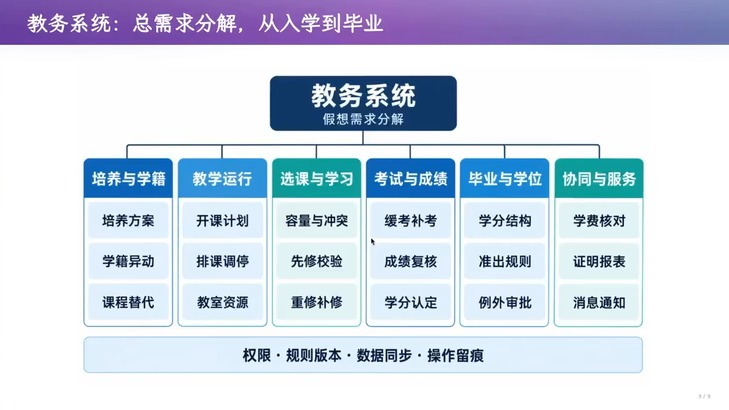
\includegraphics[width=\textwidth]{figures/fig_13_req_decomposition.jpg}
\caption{教务系统的假想总需求分解：培养与学籍、教学运行、选课与学习、考试与成绩、毕业与学位、协同与服务六大块，底部是横切的权限、规则版本、数据同步与操作留痕\vtag}
\end{figure}
\srcnote{00:32:30--00:32:44}

这张从入学到毕业的需求分解图展示了一个完整教务系统的范围。讲者对“需求”的定义很朴素：通过无尽的、与客户的沟通，把客户想要什么想清楚。小到界面上要不要放当前学期和学年、修改按钮放在哪里，都要和用户对齐，因为用户不是你自己。

\begin{warningbox}{计算机专业学生常缺的软技能：同理心}
讲者举例说，你不能因为自己是 geek，就假设所有人都会写程序。设想教务员是一位本科学历、今年 53 岁、还有两年就要退休的女士，她上大学时可能都没操作过电脑。教务系统要为她设计，也要为年轻教师设计，怎样得到一张让双方都满意的表，是完全另外的一个问题。讲者说这不是本课的重点，但它决定了需求能否对齐。
\end{warningbox}

\subsection{本章小结}

需求工程的产物是一套可讨论、可追溯、可验收的结构：业务目标、带编号的功能需求、验收口径、追踪矩阵。AI 已经能在一小时内调研出这样一份文档，并照着它实现一个像样的演示系统。这带来一个诱人的结论——只要需求写清楚，其余交给 AI。下一节讲者立刻给这个结论泼冷水：需求永远写不清，而且会变。
\section{需求的泥潭：说不清、会变、每一步都是技术债}

本节回答：既然 AI 能照着需求说明书实现系统，为什么真实的业务系统仍然会陷入泥潭？

\subsection{经典做法为什么走不通}

讲者先承认行业经验的价值：一家在教育行业摸爬滚打 20 年的公司，对学位授予流程比“毛头小伙子”清楚得多，知道教务员想要什么，也知道怎样把流程变成需求文档列表；新手做的需求则很可能有偏差。这就是行业的壁垒。

\begin{figure}[H]
\centering

\includegraphics[width=\textwidth]{figures/fig_14_req_swamp.jpg}
\caption{教务系统的需求泥潭：按经典软件工程思路把需求方访谈一遍，期末考试都结束了；学生、老师、教务员、教务处、财务、辅导员各有需求；客户说不清楚明确的需求（必修二选一、准出、先修等规则，转专业、交换、缓考、补考、课程替代等例外）；即使说清楚了也未必能达成一致\vtag}
\end{figure}
\srcnote{00:34:00--00:34:14}

但即便有经验，做软件在某种程度上也是“被迫的”。讲者的解释是：一个空项目里没有任何东西在漂移；一旦写出需求列表，AI 或人类马上就实现一版，就像上一节的演示系统一样。实现之后，你就背上了技术债，因为下面这两条定律总是成立。

\begin{importantbox}{讲者的两条需求定律}
第一，你永远不可能真的把用户的需求说清楚。第二，需求不是一成不变的。

由此推出：任何时候你实现了需求，一旦做了需求分析，你就背上了技术债。
\end{importantbox}

\subsection{案例：离散数学拆成两门之后}

讲者用一个他认为“真的可能在学校里发生”的例子说明第二条定律。南大计算机专业把原来一学期的离散数学拆成了上下两学期两门课，因为原来那门课没有教会学生数学的语言。拆课带来一个糟糕的后果：准出（毕业）要求和保研要求都变了，新旧系统衔接不上。

在旧系统里，规则是“计算机专业学生毕业必须修过离散数学”。当初写需求 checklist 时，这是非常合理的：在“毕业要求”界面上给教务员一个下拉框和一个“增加一条”按钮，选择一门必修课即可。拆课之后，这个设计就不能适应新的需求了：毕业条件要变成“修过离散数学，或者修过离散数学（一）”，这是一个“或”的关系。于是只能把需求文档调出来，在下拉框里加一个“或”。讲者说，每当你叠加一个这样的补丁，“屎山”就开始累积：你本来做了一个整体一致的设计，需求中间一旦出现裂缝，就会传递到系统的各个部分，一个看似很小的改动牵动全局。

例外还会继续出现。讲者列举了重修、交换、学分抵扣；如果一个同学从别的院系转来，那里还只有一门离散数学（讲者提到软件学院似乎仍是一门），它该抵扣计算机学院的离散数学（一）和（二），还是只抵扣（一）、再补修（二）？面对开放的物理世界，这样的情况无穷无尽。

最后总有一个“override”。假设某位同学读到第六年，恰好因为离散数学拆课拿不到学位，而春季学期才开的那门课他已经来不及修了。教学主任认定两门课之间可以替代，那系统里怎么办？最终是打电话给工程师，在数据库里把这位同学的毕业条件改成“满足”。讲者补充，这件事在人类世界里有合理的解释，层层审批的记录也还在，但它发生在系统之外。

\begin{figure}[H]
\centering
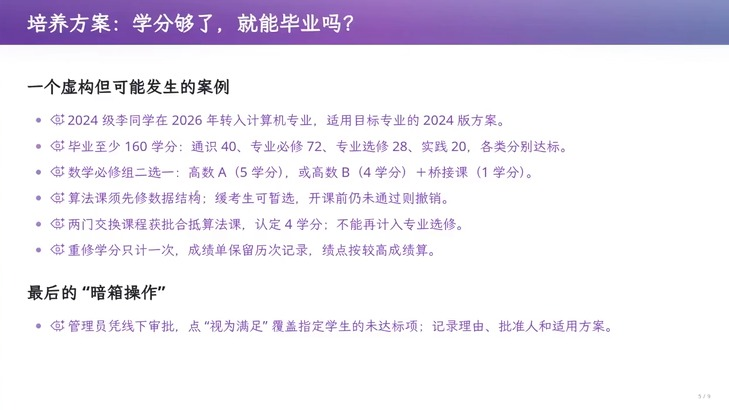
\includegraphics[width=\textwidth]{figures/fig_15_graduation_case.jpg}
\caption{“培养方案：学分够了，就能毕业吗？”——一个虚构但可能发生的案例，列出转专业、学分类别、数学二选一、先修、交换课抵扣、重修计分等规则，以及最后的“暗箱操作”：管理员凭线下审批点“视为满足”，并记录理由、批准人和适用方案\vtag}
\end{figure}
\srcnote{00:39:00--00:39:14}

幻灯片把这类规则写得更具体（下表）。每一行都是一个会穿透课程对应、学分统计、毕业审核、成绩单乃至测试用例的约束。

\begin{table}[H]
\centering
\small
\begin{tabular}{p{3.2cm}p{10.4cm}}
\toprule
规则类别 & 幻灯片上的具体规定（虚构但可能发生） \\
\midrule
适用方案 & 2024 级李同学在 2026 年转入计算机专业，适用目标专业的 2024 版方案 \\
学分构成 & 毕业至少 160 学分：通识 40、专业必修 72、专业选修 28、实践 20，各类分别达标 \\
二选一 & 数学必修组：高数 A（5 学分），或高数 B（4 学分）+ 桥接课（1 学分） \\
先修 & 算法课须先修数据结构；缓考生可暂选，开课前仍未通过则撤销 \\
抵扣 & 两门交换课程获批合抵算法课，认定 4 学分；不能再计入专业选修 \\
重修 & 重修学分只计一次，成绩单保留历次记录，绩点按较高成绩算 \\
人工覆盖 & 管理员凭线下审批点“视为满足”，覆盖指定学生的未达标项，记录理由、批准人和适用方案 \\
\bottomrule
\end{tabular}
\caption{培养方案案例中的规则（据 00:39:00 画面整理）}
\label{tab:grad}
\end{table}

\subsection{焦油坑：一个 $-1$ 让页面全部瘫痪}

讲者讲了一个亲身经历。他开始上课的第一天（他记得大约是 2018 年，当时还是老版的教务系统），第一次用教师端，发现系统可以给学生设置缺课次数。他不理解为什么要做这个需求：学生缺课，老师留一张签到表、扫描存档就足以作为处理依据，没必要进系统。于是他试着绕过前端校验，把一位同学的缺课次数从 0 改成了 $-1$，这看起来并不是什么有害的操作。

\begin{figure}[H]
\centering
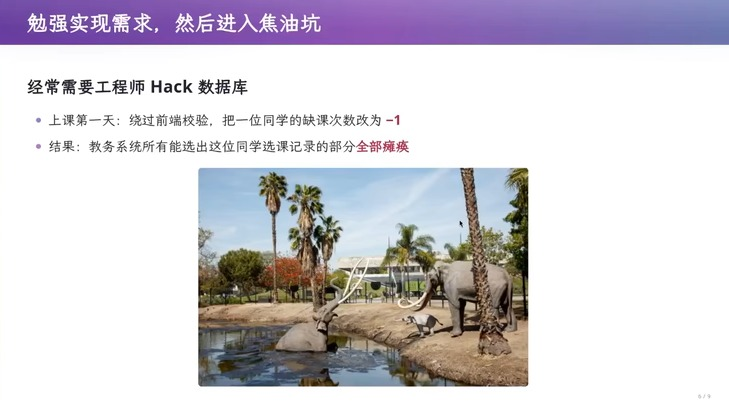
\includegraphics[width=\textwidth]{figures/fig_16_tar_pit.jpg}
\caption{勉强实现需求，然后进入焦油坑：经常需要工程师 Hack 数据库。上课第一天，绕过前端校验把一位同学的缺课次数改为 $-1$，结果教务系统所有能选出这位同学选课记录的部分全部瘫痪\vtag}
\end{figure}
\srcnote{00:40:45--00:40:59}

结果，所有能选出这位同学选课记录的页面全部崩溃，直接返回 HTTP 500。讲者只好打电话告诉教务处系统崩了；第二天大概是工程师登录数据库，把那条 $-1$ 的记录修复了。讲者说，这就是学生将来真实面对的软件系统需求。对照上一节：GPT 实现的演示系统前后端都做了校验，这是 AI 在“已写清的需求”上做得好的地方；焦油坑里的问题，是没有写清、也没人想到的那部分。

\subsection{Agentic MVP 的错觉与“没有银弹”}

讲者据此把需求定位为本课的一个引子：需求和产品设计也许应当是另一门产品课的内容，本课只讲到 Agentic AI 时代的一个判断。

\begin{figure}[H]
\centering

\includegraphics[width=\textwidth]{figures/fig_17_agentic_mvp.jpg}
\caption{Agentic AI 时代的 MVP：有用，且前所未有地容易——优先实现最重要的功能，看到产品就立即知道哪里做对、哪里做错；让客户试用也是在发现尚未说出口的需求（“这门课我已经在交换时修过了”）；Brooks 在《没有银弹》中也主张用快速原型和迭代澄清需求。但它会让你产生“驾驭了 AI”的错觉：那些 dark corners 还没有露出獠牙\vtag}
\end{figure}
\srcnote{00:42:30--00:42:44}

做 MVP 没问题，而且此时推倒重来的成本较低，迭代三个版本 AI 都能往后修。错觉在于：一旦系统在真实环境里运行得足够久——比如计算机系改成了计算机学院——原来的设计不再起作用，麻烦才真正开始。

\begin{figure}[H]
\centering
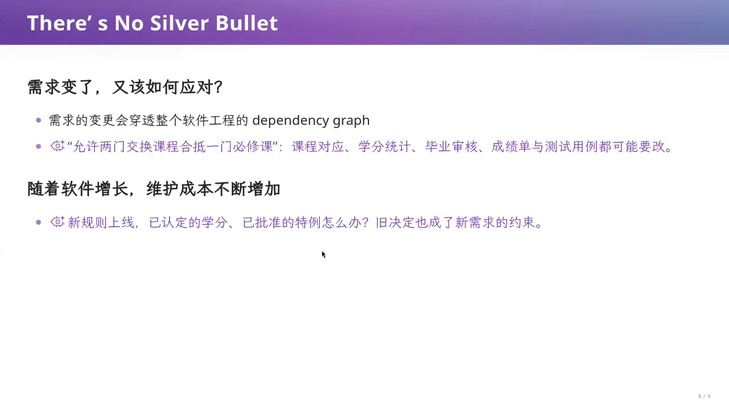
\includegraphics[width=\textwidth]{figures/fig_18_no_silver_bullet.jpg}
\caption{There's No Silver Bullet：需求的变更会穿透整个软件工程的依赖图，例如“允许两门交换课程合抵一门必修课”会波及课程对应、学分统计、毕业审核、成绩单与测试用例；随着软件增长维护成本不断增加，旧决定也成了新需求的约束\vtag}
\end{figure}
\srcnote{00:43:45--00:43:59}

\begin{knowledgebox}{背景：银弹}
西方传说中，普通子弹奈何不了狼人，只有银弹能制服它。Brooks 在 1987 年的《没有银弹》中用它比喻人们期待的“软件工程万能药”，并断言不存在这样的一招制胜。讲者把它接到本讲的主线上：软件一旦上线就开始和物理世界“交火”，为了生存和挣钱，你必须背着最初那些决策留下的技术债持续维护；前期决策越不前瞻，维护成本就越高。
\end{knowledgebox}

\subsection{本章小结}

需求文档从写出来那一刻就开始过时：用户说不清，需求会变，而每个已实现的需求都会以数据库字段、界面控件、校验规则的形式固定下来，成为下一个需求的约束。AI 让第一版变得廉价，却不会替你判断哪些决定将来会被推翻。讲者给出的出路是：在一开始，除了做 MVP，还要想软件的第一步迈向哪里最有利于长期生存——这就是架构。
\section{架构是什么：让复杂性有归处，让变化有边界}

本节回答：讲者所说的“架构”指什么，为什么说再小的代码也有架构？

\subsection{架构：驾驭复杂性，应对变化}

讲者在需求之后引出架构，并给它很高的地位：它是真正决定软件品味和能走多远的决定性因素。按幻灯片的表述，架构有两项职能：一是驾驭问题的复杂性——简化问题、安放复杂性、减少依赖；二是应对需求的变化、降低维护成本。

\begin{figure}[H]
\centering
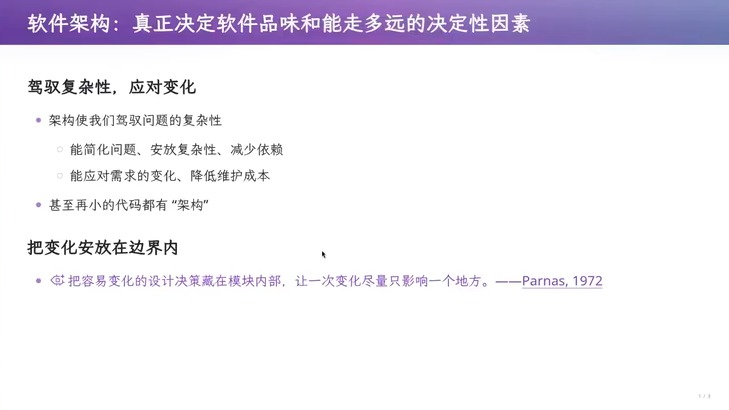
\includegraphics[width=\textwidth]{figures/fig_19_architecture_def.jpg}
\caption{软件架构：驾驭复杂性、应对变化；甚至再小的代码都有“架构”；把变化安放在边界内——把容易变化的设计决策藏在模块内部，让一次变化尽量只影响一个地方（Parnas, 1972）\vtag}
\end{figure}
\srcnote{00:44:30--00:44:44}

\begin{importantbox}{本讲对架构的工作定义}
好的架构：复杂性有归处，变化有边界（这是讲者下一页幻灯片的标题）。落到行动上，讲者说“说白了就一个：把耦合解开”。例如一开始就用一个数据库存放所有东西，你能很快得到一个能工作的原型，AI 也能很快做出来；但如果不仔细想系统里哪些概念本可以分开，就很容易掉进维护的泥潭。
\end{importantbox}

讲者也区分了 MVP 与原型：第 3 节 AI 生成的那个教务“MVP”其实已经是一个小型产品原型，维护它会变得非常困难。想驾驭复杂性，一开始要问的是：怎样做一个最小的软件，使它在需求膨胀和改变时仍有一定韧性。

\subsection{再小的代码也有架构}

讲者说，大家一谈架构就觉得是玄学、很高大上，其实不是。从你第一次设计任何代码开始，无论它多小，里面都有架构思维，因为架构本质上是控制复杂性的方式；代码哪怕只有一点点规模，你就可以考虑复杂性应该怎样分解。他举的第一个例子是很多人写 OJ 题时的结构。

\begin{figure}[H]
\centering

\includegraphics[width=\textwidth]{figures/fig_20_small_code_arch.jpg}
\caption{再小的代码也有架构：甚至最小的“状态机”就是架构；讲者不喜欢“语言律师”式的授课，语义的价值是把设计意图变成约束，并请读者回看这四个函数——数据怎样穿过各阶段、换一种输入格式需要改到哪里\vtag}
\end{figure}
\srcnote{00:47:00--00:47:14}

\begin{lstlisting}[language=C, caption={最小的架构：把程序分成读入、解析、处理、输出四个阶段（幻灯片代码）}]
int main() {
    read_input();
    parse_input();
    process_input();
    write_output();
}
\end{lstlisting}

这四个函数把“数据如何穿过各阶段”固定成一条流水线。幻灯片提出的检验问题正是架构的检验：如果换一种输入格式，需要改到哪里？在这个结构下，答案应当是只改 \texttt{read\_input} 和 \texttt{parse\_input}，处理与输出不受影响——变化被关在了边界之内。

\subsection{getopt：把 argv 的复杂性隔离成解析状态}

第二个例子是命令行参数。\texttt{main} 函数的 \texttt{argc} 与 \texttt{argv} 是操作系统和进程之间的约定：参数以字符串向量的形式传进来。讲者问：如果保研机试要求处理 argv，你会逐个 \texttt{strcmp} 吗？argv 本身很复杂：有短参数，有 Unix 风格的长参数，有的带值有的不带；在 C 的时代手写一个解析器很麻烦。更好的做法是想起 \texttt{getopt}：这套参数约定有 POSIX 标准，按标准就能用 \texttt{getopt} 处理，最后只剩一个 \texttt{while} 循环加一个 \texttt{switch}。讲者现场用 \texttt{man 3 getopt} 展示了它的原型（\texttt{getopt}、\texttt{getopt\_long}、\texttt{getopt\_long\_only}），并对照 \texttt{eza} 等工具的大量长参数说明这种复杂性真实存在。

\begin{lstlisting}[language=C, caption={getopt 的典型用法（本讲义据讲者“while 循环加 switch”的描述补写，选项名为示意）}]
#include <unistd.h>

int main(int argc, char *argv[]) {
    int opt, verbose = 0;
    const char *out = NULL;
    while ((opt = getopt(argc, argv, "vo:")) != -1) {
        switch (opt) {
            case 'v': verbose = 1; break;      /* flag */
            case 'o': out = optarg; break;     /* option with a value */
            default:  return 1;                /* unknown option */
        }
    }
    /* from here on, only the parsed state (verbose, out) matters */
}
\end{lstlisting}

讲者的解读是：这种“parsing 的模式”把一个复杂的字符串变成一个简单的解析状态（parsing state），后续逻辑只依赖这个状态。argv 可以有各种变化，但这些变化都被关在解析这一层，因此它本身就是一种抵抗需求变化的方式。讲者说，你在任何符合 best practice 的代码背后都能看到架构设计，而架构又都映射到需求；在任何一个模块里，都可以谈 intent、specification 和 implementation，都可以谈需求、架构和优雅，并不只有教务系统那样的巨型单体才需要。

\begin{warningbox}{讲者批评的教学方式：只教语法，不教意图}
讲者说，他曾和学院的老教师在 C++ 教学上有较大分歧：他希望讲 C++11/17 的一些特性以及它们应该怎么用，对方回应“我讲了”，讲的却是“Lambda 就是 \texttt{[](a, b)} 返回 \texttt{a + b}”，没有了。讲者认为这和没讲没有区别。你学的每一个语法、库函数，都可能和架构有千丝万缕的联系；按幻灯片的说法，语义的价值在于把设计意图变成约束：谁能改数据，谁负责资源，谁可以依赖谁。只背语法规则的“语言律师”式教学，恰好丢掉了这部分。
\end{warningbox}

\subsection{本章小结}

架构是任何代码里“复杂性放在哪里、变化被关在哪里”的决定，再小的程序也有。四阶段的 \texttt{main} 和 \texttt{getopt} 都在做同一件事：用一个稳定的中间形态（流水线阶段、解析状态）把易变的输入与后续逻辑隔开。讲者接着说明，为什么今天的模型在架构上还不够好：架构和需求连在一起，好架构取决于你对需求掌控到什么程度。下一节用一个 10 行的例子展示这一点。
\section{10 行的架构：非递归汉诺塔的四种写法}

本节回答：同一个 10 行规模的问题，不同的“作者”会把复杂性放在哪里，这和对需求的掌控有什么关系？

\subsection{问题：为什么大家写不出非递归汉诺塔}

\begin{figure}[H]
\centering
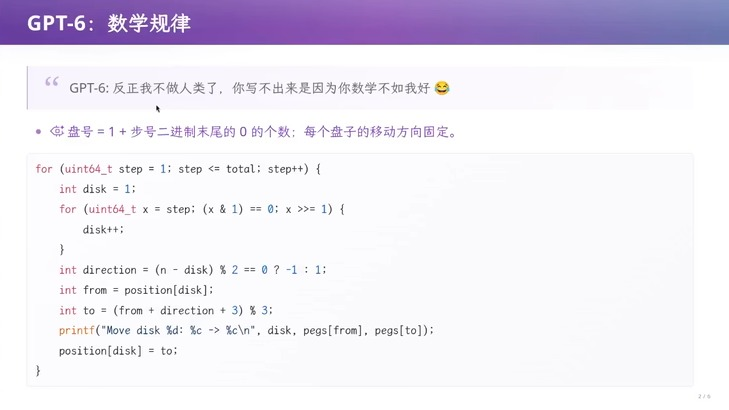
\includegraphics[width=\textwidth]{figures/fig_21_hanoi_gpt6.jpg}
\caption{GPT-6 的非递归汉诺塔：“反正我不做人类了，你写不出来是因为你数学不如我好”——盘号 = 1 + 步号二进制末尾的 0 的个数，每个盘子的移动方向固定\vtag}
\end{figure}
\srcnote{00:52:30--00:52:44}

讲者说这是他最喜欢的例子。他以前问保研来的研究生能不能写出非递归的汉诺塔（Tower of Hanoi），研究生摇头，这个问题于是成了他上课的例子。幻灯片的标题是“架构关乎你对需求‘掌控到什么程度’”，并引用了 Zhang 与 Norman 1994 年的研究：同一个问题换一种表示，难度就可能改变，汉诺塔的同构变体实验也观察到了这种差异。讲者把同一个 prompt（写一个非递归汉诺塔）交给不同的模型，再给出自己的写法。

\subsection{GPT-6：把递归树压缩成数学规律}

GPT-6 找到了汉诺塔的数学性质。讲者转述它的态度是“我不做人类了”，并判断它“应该是对的”，只是人看不明白，但高度优化。代码的核心是一个数学关系：

\[
d(s) = 1 + \operatorname{tz}(s)
\]

\begin{itemize}
  \item $s$：步号，从 1 开始计数；
  \item $\operatorname{tz}(s)$：$s$ 的二进制表示末尾连续 0 的个数；
  \item $d(s)$：第 $s$ 步要移动的盘号（1 为最小的盘）。
\end{itemize}

盘子的移动方向也由公式给出（取自幻灯片代码）：

\[
\mathit{dir}(d) = \begin{cases} -1, & (n-d)\bmod 2 = 0 \\ +1, & \text{否则} \end{cases}
\qquad
\mathit{to} = (\mathit{from} + \mathit{dir}(d) + 3) \bmod 3
\]

\begin{itemize}
  \item $n$：盘子总数；$d$：本步移动的盘号；
  \item $\mathit{dir}(d)$：盘 $d$ 固定的移动方向，在三根柱子上循环前进或后退一格；
  \item $\mathit{from}$、$\mathit{to}$：盘 $d$ 当前所在柱子与目标柱子的编号（0、1、2），$+3$ 用来避免负数取模。
\end{itemize}

\begin{lstlisting}[language=C, caption={GPT-6 的写法：按步号计算盘号与方向（幻灯片代码）}]
for (uint64_t step = 1; step <= total; step++) {
    int disk = 1;
    for (uint64_t x = step; (x & 1) == 0; x >>= 1) {
        disk++;
    }
    int direction = (n - disk) % 2 == 0 ? -1 : 1;
    int from = position[disk];
    int to = (from + direction + 3) % 3;
    printf("Move disk %d: %c -> %c\n", disk, pegs[from], pegs[to]);
    position[disk] = to;
}
\end{lstlisting}

\subsection{DeepSeek：把递归展开成显式任务栈}

讲者说，同样的 prompt 下 DeepSeek V4 Flash“更有人感”：它写出的基本就是标准答案，一个非常干净的架构。它理解递归的本质：要把一堆盘子移过去时，剩下还要继续执行的任务必须留在栈里，于是总是执行栈顶的任务。讲者还试了豆包，它选了同样的方案，但写出的代码有瑕疵，讲者没有展示。

\begin{figure}[H]
\centering
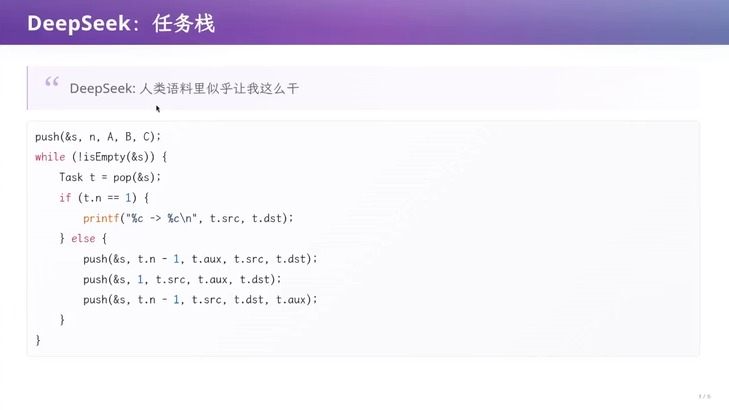
\includegraphics[width=\textwidth]{figures/fig_22_hanoi_deepseek.jpg}
\caption{DeepSeek 的非递归汉诺塔：“人类语料里似乎让我这么干”——用显式任务栈保存尚未完成的子任务\vtag}
\end{figure}
\srcnote{00:53:00--00:53:14}

\begin{lstlisting}[language=C, caption={DeepSeek 的写法：任务栈（幻灯片代码；因栈后进先出，三个子任务逆序压栈）}]
push(&s, n, A, B, C);
while (!isEmpty(&s)) {
    Task t = pop(&s);
    if (t.n == 1) {
        printf("%c -> %c\n", t.src, t.dst);
    } else {
        push(&s, t.n - 1, t.aux, t.src, t.dst);
        push(&s, 1, t.src, t.aux, t.dst);
        push(&s, t.n - 1, t.src, t.dst, t.aux);
    }
}
\end{lstlisting}

\subsection{讲者的写法：把 C 语言的执行机制显式化}

讲者说，作为架构师，他想的是另一个问题：大家为什么写不出来？因为对“递归”这件事理解得不够深。他在操作系统课上花了一整节课讲过：程序是一个状态机，C 语言有自己的状态，单步执行的规则就是它的操作语义（operational semantics）；像 \texttt{hanoi(n-1, ...)} 这样的一步，在程序语言的意义上是良定义的。所以只要模拟这个状态机——本质上写一个小小的 C 解释器——就能把任何递归代码（包括 \texttt{f} 调 \texttt{g}、\texttt{g} 又调 \texttt{f} 的互递归）机械地翻译成非递归形式，没有任何难度。

\begin{figure}[H]
\centering
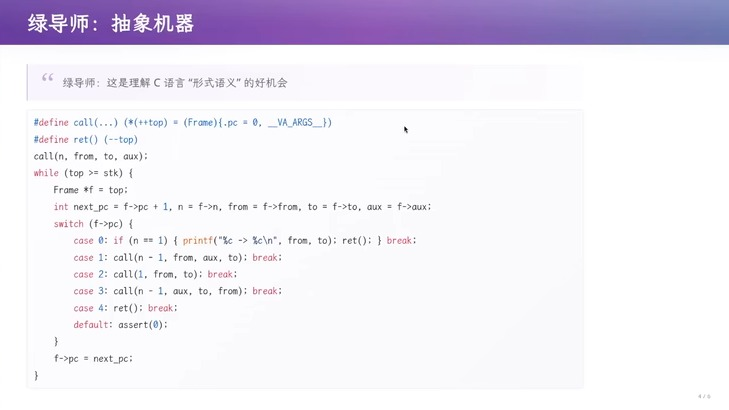
\includegraphics[width=\textwidth]{figures/fig_23_hanoi_abstract_machine.jpg}
\caption{讲者（“绿导师”）的写法：这是理解 C 语言“形式语义”的好机会——用 \texttt{call}/\texttt{ret} 宏维护栈帧，每帧保存参数与程序计数器 \texttt{pc}\vtag}
\end{figure}
\srcnote{00:54:15--00:54:29}

\begin{lstlisting}[language=C, caption={抽象机器写法：栈帧里的 pc 记录“这次调用执行到哪一步”（幻灯片代码）}]
#define call(...) (*(++top) = (Frame){.pc = 0, __VA_ARGS__})
#define ret()     (--top)

call(n, from, to, aux);
while (top >= stk) {
    Frame *f = top;
    int next_pc = f->pc + 1, n = f->n, from = f->from, to = f->to, aux = f->aux;
    switch (f->pc) {
        case 0: if (n == 1) { printf("%c -> %c\n", from, to); ret(); } break;
        case 1: call(n - 1, from, aux, to); break;
        case 2: call(1, from, to); break;
        case 3: call(n - 1, aux, to, from); break;
        case 4: ret(); break;
        default: assert(0);
    }
    f->pc = next_pc;
}
\end{lstlisting}

讲者承认，对汉诺塔来说这个写法 overkill，因为它能翻译任意程序；对它做一些化简和优化，就能得到 DeepSeek 那样的任务栈版本，两者是等价的。讲者对 GPT 的判断是：它可能其实懂，只是不会往这个方向想；他比较有信心强化学习能把模型引导到这个方向，学会之后它也会在适当的时候写出这样的实现。

最后是一个反面例子：讲者在搜索引擎里搜“非递归汉诺塔”，排第一的结果仍然是递归版，往下找到的一篇博客代码逐个枚举分支，问题比 AI slop 还严重，评论区却是一片“干货满满”的好评。讲者提醒，学习时如果被这种内容污染，还不如直接跟 AI 学。

\subsection{四种表达，复杂性放在了哪里}

\begin{figure}[H]
\centering
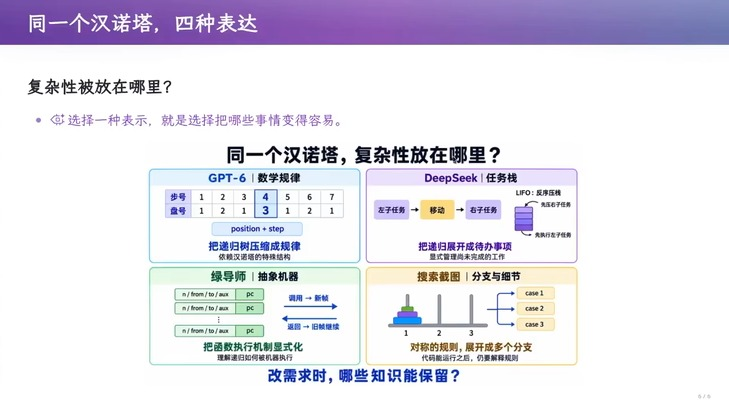
\includegraphics[width=\textwidth]{figures/fig_24_hanoi_four_forms.jpg}
\caption{同一个汉诺塔，四种表达：复杂性被放在哪里？选择一种表示，就是选择把哪些事情变得容易；改需求时，哪些知识能保留？\vtag}
\end{figure}
\srcnote{00:56:45--00:56:59}

\begin{table}[H]
\centering
\small
\begin{tabular}{p{2.6cm}p{4.4cm}p{6.4cm}}
\toprule
写法 & 把复杂性放在哪里 & 幻灯片的评语 \\
\midrule
GPT-6：数学规律 & 盘号与步号的数学关系 & 把递归树压缩成规律；依赖汉诺塔的特殊结构 \\
DeepSeek：任务栈 & 显式的待办任务栈 & 把递归展开成待办事项；显式管理尚未完成的工作 \\
讲者：抽象机器 & 栈帧与程序计数器 & 把函数执行机制显式化；理解递归如何被机器执行 \\
搜索结果：分支与细节 & 逐个枚举的分支 & 对称的规则展开成多个分支；代码能运行之后仍要解释规则 \\
\bottomrule
\end{tabular}
\caption{同一个汉诺塔的四种表达（据 00:56:45 画面整理）}
\end{table}

\begin{importantbox}{跳出问题看问题}
讲者把这四种写法归结为站在不同层面看同一个问题。GPT-6 跳到数学层面：一切都是数学规律。DeepSeek 在语料里学到“递归就是栈”，做了一个正确的实现。讲者又往外走了一步：把对编程语言世界的理解（递归与非递归的区别来自执行机制）投射成代码。幻灯片最后的问题是“改需求时，哪些知识能保留”。本讲义据讲者“可以把任意程序翻译成状态机”的说法整理为：如果需求从汉诺塔换成另一个递归问题，依赖汉诺塔特殊结构的数学规律几乎无法复用，抽象机器的翻译方法则可以照搬。架构水平的高低，在 10 行代码里就能看出来。
\end{importantbox}

\subsection{本章小结}

同一个 10 行的问题可以有截然不同的架构，差别在于作者把复杂性放在了哪个层面。讲者用它说明“架构关乎你对需求掌控到什么程度”：理解得越深，越能选出一种在需求变化时仍能保留知识的表示。下一节把尺度放大到 2000 行：一个需求看起来完全明确的 Excel 二维码生成器。
\section{2000 行的架构：Excel 二维码生成器其实是个编译器}

本节回答：一个需求看上去完全明确的任务，为什么仍然需要架构？“跳出问题看问题”在 2000 行规模上长什么样？

\subsection{需求明确，实现却极长且脆弱}

讲者在课程第一讲演示过一个例子：在 Excel 里生成二维码。一个单元格输入任意字符串，另一组单元格输出由 0 和 1 组成、可以直接扫描的二维码。和教务系统不同，它的需求非常明确，是一个完全确定性（deterministic）的任务。

讲者先观察到 Agent 对自己的能力有估计。比如给它两个工作表，一张是期末考试成绩，一张是实验成绩，让它写公式按学号把实验成绩拉过来，这在它的能力范围内，它会一把写出。二维码这件事显然超出了它的能力范围，它会试图分解问题，也会做一些架构，但讲者认为至少今天的模型在架构上“稍稍有些落后”。

\begin{figure}[H]
\centering
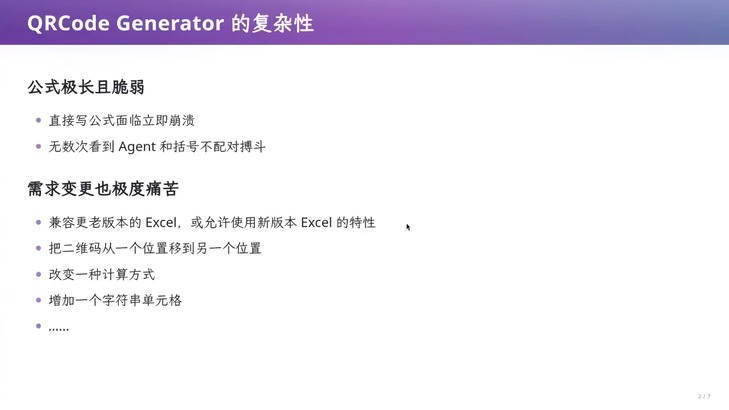
\includegraphics[width=\textwidth]{figures/fig_25_qr_complexity.jpg}\\[4pt]
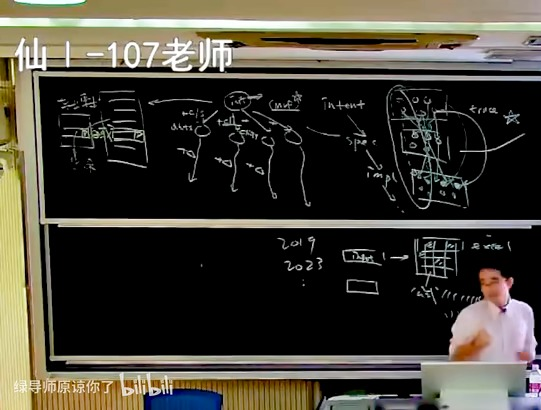
\includegraphics[width=0.72\textwidth]{figures/fig_25_board_excel_versions.jpg}
\caption{上：QRCode Generator 的复杂性——公式极长且脆弱（直接写公式面临立即崩溃，无数次看到 Agent 和括号不配对搏斗）；需求变更也极度痛苦（兼容更老版本的 Excel 或允许新版本特性、把二维码从一个位置移到另一个位置、改变计算方式、增加一个字符串单元格）。下：同一时刻的板书，左侧写着 2019、2023 两个 Excel 版本，右侧是输入单元格与二维码网格\vtag}
\end{figure}
\srcnote{01:02:15--01:02:29}

直接把算法写成一个公式会发生什么？讲者引了一个老笑话：有人偷到了国防部的 Lisp 程序，最后一页全是右括号。Excel 的计算能力有限，用它写二维码，好比用 Brainfuck 去实现一个非平凡的程序，写出来就是那样。更麻烦的是这个“明确”的需求其实有很多坑：

\begin{itemize}
  \item \textbf{版本}：Excel 一直在演化。按学号查成绩，以前用 \texttt{VLOOKUP}，后来微软推出了更方便的 \texttt{XLOOKUP}。那么该兼容旧版本，让发给教务老师的文件也能打开，还是只给自己一次性使用、直接用最新语法写最简单的公式？如果 AI 用 2023 版的公式写好了，你突然说要改成 2019，甚至 2003，那就是摧毁性的：设计和实现回到原点。
  \item \textbf{位置}：做完之后你对二维码的位置不满意，想整体往右移一格；如果所有单元格都是硬编码的，就立即崩溃。
\end{itemize}

对一个独立的 2000 行项目，大不了重做；但如果它已经嵌进教务系统那样巨大的需求里、与其他部分产生了关联，讲者说那就只能“加钱”了。这显然是架构没有设计好：它对需求变更的抵抗力很差。

\subsection{跳出问题看问题：二维码本来就容易用算法描述}

讲者让 Agent 给出一份“从字符串到二维码的伪代码”。结果非常短：

\begin{figure}[H]
\centering
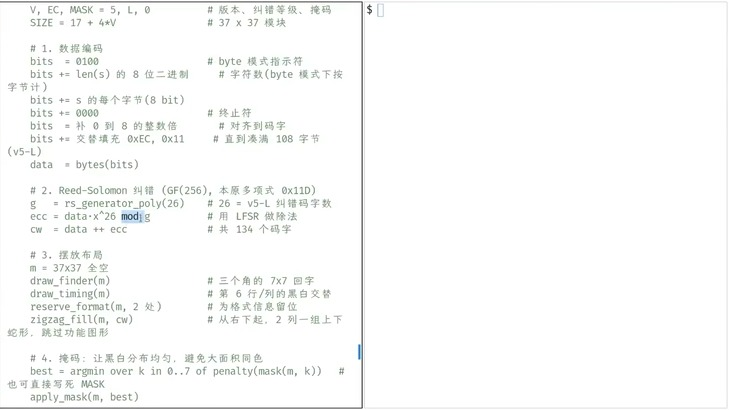
\includegraphics[width=\textwidth]{figures/fig_26_qr_pseudocode.jpg}
\caption{Agent 给出的二维码伪代码：版本 5、纠错等级 L、37×37 模块；数据编码、Reed–Solomon 纠错、摆放布局、掩码四步\vtag}
\end{figure}
\srcnote{01:05:45--01:05:59}

伪代码里有两个关键的数量关系。第一个决定二维码的尺寸：

\[
\mathit{SIZE} = 17 + 4V
\]

\begin{itemize}
  \item $V$：二维码版本号，这里取 $V=5$；
  \item $\mathit{SIZE}$：每边的模块数，$V=5$ 时为 $17+20=37$，即 37×37 模块。
\end{itemize}

第二个是纠错码的计算：

\[
\mathit{ecc} = \mathit{data}\cdot x^{26} \bmod g, \qquad \mathit{cw} = \mathit{data} \,\|\, \mathit{ecc}
\]

\begin{itemize}
  \item $\mathit{data}$：数据码字构成的多项式（版本 5-L 下数据补齐到 108 字节）；
  \item $g$：Reed–Solomon 生成多项式，\texttt{rs\_generator\_poly(26)}，26 是 5-L 的纠错码字数；运算在 GF(256) 上进行，本原多项式为 \texttt{0x11D}，伪代码注释说用 LFSR 做除法；
  \item $\mathit{ecc}$：余式，即 26 个纠错码字；
  \item $\mathit{cw}$：数据与纠错码字拼接，共 134 个码字（$108+26$）。
\end{itemize}

其余步骤是：数据编码（byte 模式指示符 \texttt{0100}、8 位字符数、每个字节、终止符 \texttt{0000}、补 0 对齐、交替填充 \texttt{0xEC}、\texttt{0x11}）；摆放布局（三个角的 7×7 定位图案、第 6 行/列的黑白交替时序图案、为格式信息留位、从右下起两列一组上下蛇形填充）；掩码（在 8 种掩码里选惩罚最小的，也可以直接写死）。讲者说，把它写成一个 \texttt{qr.py} 再容易不过，甚至可以作为保研机试题。

那么 gap 在哪里？讲者的回答是：二维码容易用算法描述，但我们的要求是 Excel，而世界上不存在把 Python 编译成 Excel 的编译器——Excel 本来是为财务报表、成绩管理这类小数据库设计的，不是为图灵完备的计算设计的。如果把伪代码或自然语言直接交给大模型去“编译”，它会直接上手做，需求一漂移就遇到前面那些问题。

\subsection{中间语言：一份计算图，两个后端}

\begin{figure}[H]
\centering

\includegraphics[width=\textwidth]{figures/fig_27_qr_compiler.jpg}
\caption{我们其实要实现的是“编译器”：二维码算法容易用伪代码/编程语言描述，但不能原样变成 Excel 公式；先用中间语言（IR）表达计算规则，再决定怎样落到 Excel 上；用 Python 的函数和循环构造计算图，字符串输入保留为符号，输入决定的分支写成 \texttt{Select(cond, a, b)} 节点\vtag}
\end{figure}
\srcnote{01:06:45--01:06:59}

讲者的设计是在 Python 和 Excel 之间构造另一种语言。它既能容易地翻译成 Excel，又能继承一部分 Python 的表达能力。讲者用学生都写过的表达式求值程序解释：一棵表达式树，节点可以是加法 \texttt{+(a, b)}，也可以是“取出字符串中某一位”之类的操作。把树递归地“dump”出来——翻译左子树、右子树，再按节点类型拼起来——就得到 Python 代码；只要为每种节点再规定一条翻译成 Excel 的规则（结果放进某个格子，再在另一个格子里组合两个格子的结果），同一棵树也能翻译成 Excel。

\begin{figure}[H]
\centering
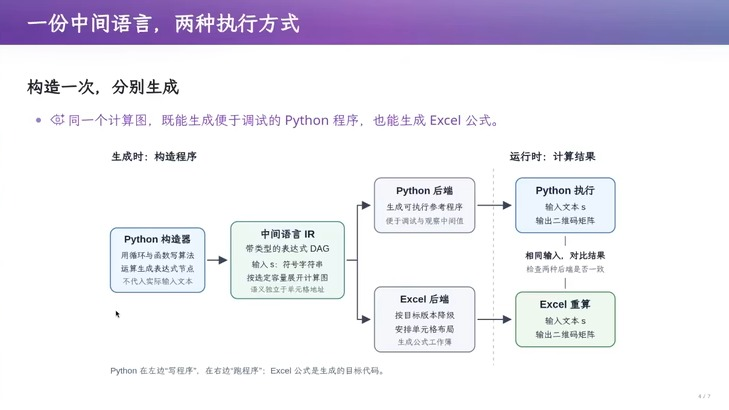
\includegraphics[width=\textwidth]{figures/fig_28_ir_two_backends.jpg}\\[4pt]
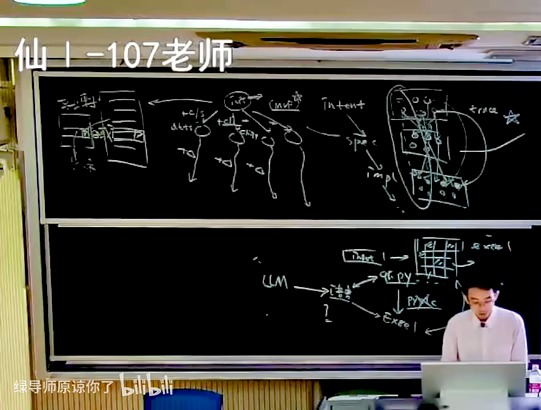
\includegraphics[width=0.72\textwidth]{figures/fig_28_board_llm_ir_excel.jpg}
\caption{上：一份中间语言，两种执行方式——生成时由 Python 构造器生成带类型的表达式 DAG（输入 $s$ 为符号字符串，语义独立于单元格地址），再由 Python 后端生成便于调试的参考程序、由 Excel 后端按目标版本降级并安排单元格布局；运行时用相同输入对比两种后端的结果。下：板书中的同一架构，LLM 生成中间语言，翻译成 qr.py 用于验证，翻译成 Excel 用于交付\vtag}
\end{figure}
\srcnote{01:10:45--01:10:59}

这样工作流程就清楚了：让大模型生成这种中间语言表达的二维码计算逻辑；先翻译成 Python 去验证公式对不对；对了之后再生成 Excel。讲者把它和第 5 节的 \texttt{getopt} 类比：写命令行工具时第一件事是 \texttt{getopt} 得到解析状态，再从那个状态出发做下一步——两者是同一种设计。

\begin{importantbox}{讲者的判断：好的架构承载需求变化}
在这个架构上，AI 生成的 slop 本身不再重要，因为它被限定在一门小语言里，并由 Python 后端交叉验证。需求变化也有了归处：Excel 版本改了，只需要把一些算子换一种方式实现（降级）；二维码要挪位置，改的是 Excel 后端的单元格布局，而不是计算逻辑。
\end{importantbox}

\subsection{性能优化也有自己的位置}

有了中间语言，优化也有了明确的位置。讲者说，如果觉得某处生成的代码太长、性能不好，就可以定义改写规则，把程序从一种形态改写成另一种形态。例如循环里每次都算、但值不变的表达式，编译器可以自动提到循环外面；你也可以手动做，或者让大模型在中间语言上做。计算机系统课里学的 Profile-Guided Optimization（先测出性能瓶颈，再用 profile 指导代码怎么写）在这里也用得上。

\begin{figure}[H]
\centering

\includegraphics[width=\textwidth]{figures/fig_29_perf_optimization.jpg}
\caption{性能优化也有自己的位置：先优化计算图（常量折叠、公共子表达式、公式内用 \texttt{LET} 复用、跨公式或旧版本用辅助单元格），再按 Excel 的实际计算成本决定内联还是拆格，并分别测量首次完整计算与修改输入后的重算时间\vtag}
\end{figure}
\srcnote{01:11:00--01:11:14}

\begin{knowledgebox}{与编译器、AI Infra 的类比}
幻灯片上的优化手段都是编译器的标准做法：常量折叠把固定参数下的定位图案、有限域常量表在生成时算好；公共子表达式让相同的纯计算在图中共享一个节点，避免反复粘贴成长公式。讲者还指出，今天做 AI Infra 的人在算子层面也在做类似的事：同一份计算图，针对不同硬件用不同方式实现算子。
\end{knowledgebox}

\subsection{架构的能力从哪里来}

讲者在进入二维码例子之前，把“跳出问题看问题”推广成一串同心圆：代码之外有客户的规律，客户之外有社会的规律，社会之外有宇宙的规律。学生自然会问：这种能力从哪来？

讲者的回答是：从你学过的每一样东西里来。如果一样东西是好的、优雅的，它会促使你思考这个问题；“压缩就是智能”，把学到的东西压缩成第一性原理，遇到新问题时总从第一性原理推导应该怎么做。他把学生比作无监督学习的神经网络：看好的东西看多了，自然就能泛化，但要有意识地去问“为什么要这样”；也许某天读到一篇博客、听到一节课，突然就想通了，发现大家做的事情其实都差不多。幻灯片上还有一句半开玩笑的话：如果有一天这个能力能被强化学习学会，就真的见证人类完蛋了。

这种能力也来自课本和做题之外的社会积累。讲者再次回到那位快退休的教务老师：你的想法总是最好的数据库、最高的性能，而她可能只想要字大一点，点鼠标时不要手滑点到旁边的按钮上。共情别人的能力，同样是架构能力的一部分。

\subsection{本章小结}

二维码生成器的需求是明确的，难点在于实现语言（Excel）与问题的自然表达（算法）之间有巨大落差，而“兼容哪个版本”“放在哪里”这些看似次要的需求随时会变。直接让 AI 写公式，等于把全部复杂性堆在一团公式里；引入中间语言，则把“算什么”“在哪个后端怎么算”“怎么优化”分到三个层次，变化各有边界。下一节进入最大的尺度：50 万行的教务系统。
\section{50 万行的架构：教务系统与 CRUD 的困境}

本节回答：一个 50 万行规模的教务系统，常见的 CRUD 架构哪里好、哪里会在需求变化时崩溃？

\subsection{先看 AI 搓出来的教务 MVP}

讲者说，一提“架构”，大家马上想到框图、数据库、微服务、流式数据处理、应用框架，好像选对几个框架就能解决教务系统的问题。在讨论架构之前，他先看了 AI 实际实现了什么。第 3 节那个只凭需求说明书实现的演示系统，打开源码是一个单体：讲者口述是一个约 53\,KB 的 \texttt{.tsx} 和一个约 38\,KB 的 services 文件。GPT 生成过程中曾写出极长的单行函数，后来它“很贴心地”用格式化工具整理过，现在看起来正常一些。

讲者随后另开一个独立会话，问“这个软件能维护吗”。GPT-6 Astra（xhigh 推理档）的回答是：能维护，但现在是把业务逻辑挤在几个大文件里的演示原型；再不拆分和统一规则，新增功能就会越来越像拆盲盒。讲者又让 Agent 评价这个系统的架构：

\begin{figure}[H]
\centering
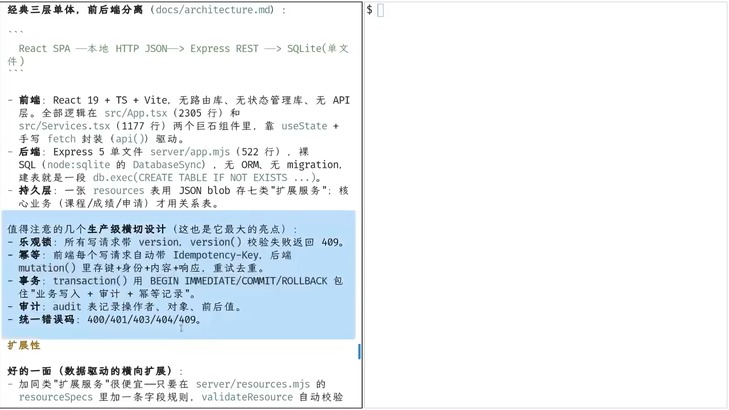
\includegraphics[width=\textwidth]{figures/fig_30_ai_arch_review.jpg}
\caption{Agent 对 AI 生成教务 demo 的架构评价：经典三层单体、前后端分离（React SPA → 本地 HTTP JSON → Express REST → SQLite 单文件）；前端逻辑集中在 \texttt{src/App.tsx}（2305 行）和 \texttt{src/Services.tsx}（1177 行），后端是单文件 \texttt{server/app.mjs}（522 行）；并列出几个生产级横切设计\vtag}
\end{figure}
\srcnote{01:15:45--01:15:59}

\begin{table}[H]
\centering
\small
\begin{tabular}{p{2.4cm}p{11.2cm}}
\toprule
横切设计 & Agent 的描述（据画面整理） \\
\midrule
乐观锁 & 所有写请求带 version，校验失败返回 409 \\
幂等 & 前端每个写请求自动带 Idempotency-Key，后端保存“键 + 身份 + 内容 + 响应”，重试时去重 \\
事务 & 用 \texttt{BEGIN IMMEDIATE/COMMIT/ROLLBACK} 包住“业务写入 + 审计 + 幂等记录” \\
审计 & audit 表记录操作者、对象、前后值 \\
统一错误码 & 400/401/403/404/409 \\
扩展性（好） & 加一类同构的“扩展服务”只需在 \texttt{resourceSpecs} 里加一条字段规则，自动校验 \\
扩展性（差） & 业务规则按申请类型硬编码成 if/else；加新申请类型或多级、并行、可配置审批要改后端、状态机和前端；JSON blob 资源表无法按字段查询、没有版本历史 \\
\bottomrule
\end{tabular}
\caption{AI 生成教务 demo 的横切设计与扩展性（01:15:45--01:16:15 画面）}
\end{table}

讲者的反应是“惊了”：这些乐观锁、幂等、事务、审计、统一错误码的设计，学生至少要摸爬滚打几年才能理解，AI 却有这种软件工程的直觉。他预期 AI 生产软件的方式很快就会超过人类。但他随即说，跳出问题看问题，这还不是一个非常好的架构，因为它本质上是一个 CRUD 架构。

\subsection{CRUD：用“当前状态”描述整个世界}

\begin{figure}[H]
\centering

\includegraphics[width=\textwidth]{figures/fig_31_crud.jpg}
\caption{CRUD 架构：用“当前状态”描述整个世界——任何时候系统都存在一个当前状态的快照（学生、教师、选课……），《数据库》课要求消除表中的冗余（normal form）以防止不一致；为每个需求点写一个状态查询/修改的业务逻辑；“Everything is a state machine”的诱惑。引语：架构是一种看待问题的方式\vtag}
\end{figure}
\srcnote{01:18:15--01:18:29}

CRUD 即增、删、改、查（Create、Read、Update、Delete）。讲者说它来自一个基本原理：软件是物理世界过程在信息世界里的投影，物理世界有状态，“everything is a state machine”，所以软件系统很自然地被建模成状态迁移系统。持久化的状态存在数据库里：一张表表示学生（学号、姓名、院系……），另外的表表示学院、选课，等等。

数据库课还要求把表分解成范式（normal form），消除冗余。讲者的例子是：另一张表引用学生时，不要用姓名，因为可能重名；就算不重名，学生改名在中国也是合法的。更好的做法是只存学生 ID（比如 1234），它像一个链接指向学生的信息，改名时只改一处，再记一个曾用名即可；如果两处都存了名字，就得两处一起改。这相当于铲除冗余的依赖。

\begin{figure}[H]
\centering

\includegraphics[width=\textwidth]{figures/fig_33_lossy_projection.jpg}\\[4pt]
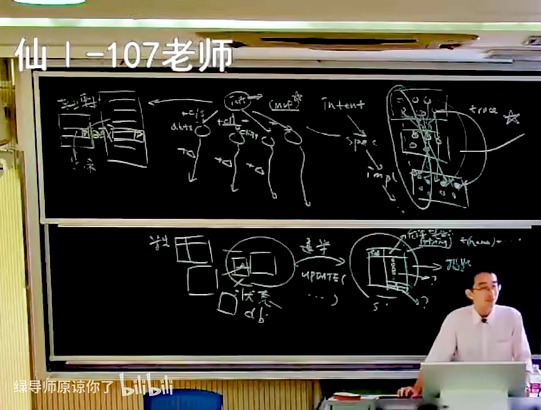
\includegraphics[width=0.72\textwidth]{figures/fig_33_board_crud_state.jpg}
\caption{上：软件是现实过程的有损投影——政策更新、领导批准还没进入教务系统时，只能在系统里 hack 成满足毕业条件，系统中不一致的数据随时间变成无法解释的黑洞；应把“例外”也变成可表达的业务，记录谁批准了哪项豁免、适用于谁、依据什么，而不是只留下 \texttt{can\_graduate = true}。下：板书中的 CRUD 模型，学生、院系等表构成当前状态，“退学”是一次 \texttt{UPDATE}，把数据库迁移到下一个状态\vtag}
\end{figure}
\srcnote{01:23:30--01:23:44}

在这个模型里，任何时刻的状态代表“此刻南京大学有哪些学生、谁选了哪些课、有哪些老师”。前后端分离的系统里，某人退学就是一次数据库 \texttt{UPDATE}：状态迁移到下一个，那个学生的记录不再存在。你打开网页看到的，永远是这个一致视图的一个投影。讲者强调，这是非常经典的架构，本身没有错误。

\subsection{CRUD 的灾难：当前状态里混着事实、规则和决定}

问题在于：看当前状态时一片祥和，但它的历史全丢了。

\begin{figure}[H]
\centering
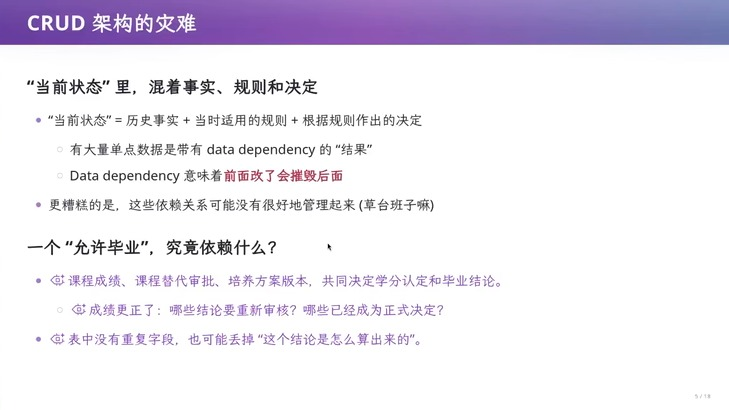
\includegraphics[width=\textwidth]{figures/fig_32_crud_disaster.jpg}
\caption{CRUD 架构的灾难：“当前状态”里混着事实、规则和决定；大量单点数据是带有数据依赖的“结果”，前面改了会摧毁后面，而这些依赖可能没有被好好管理（“草台班子嘛”）；一个“允许毕业”究竟依赖什么\vtag}
\end{figure}
\srcnote{01:21:00--01:21:14}

幻灯片把问题写成一个等式：

\[
\text{当前状态} = \text{历史事实} + \text{当时适用的规则} + \text{根据规则作出的决定}
\]

\begin{itemize}
  \item 历史事实：已经发生、不会再变的事，如某门课的成绩、某次审批；
  \item 当时适用的规则：做决定那一刻有效的培养方案版本、替代规则等；
  \item 根据规则作出的决定：由前两者算出的结论，如“允许毕业”；
  \item 等式右边三项在 CRUD 的一张表里被压成同一个字段，左边看不出右边。
\end{itemize}

讲者的例子是学生表里的一列“是否允许毕业”。这个 1 是由很多其他状态算出来的：每修一个学分、毕业设计状态每改变一次，都要重新计算一次毕业逻辑。它对信息系统很重要，因为辅导员要在系统里导出“到现在还毕不了业的学生”名单，挨个谈话，这是一个典型的需求点。但它是历史上一连串计算的依赖结果，而当前状态只保留了结果：你知道这个学生可以毕业，却不知道他为什么可以；知道他不能毕业，也不知道为什么不能。计算过程丢掉了。幻灯片追问：成绩更正了，哪些结论要重新审核？哪些已经成为正式决定？讲者还指出，现实中即使做了范式分解，也常有人把“授予某某（学号）……”之类的字符串直接写进数据库，而不用关联，数据库内部于是出现不一致。

\subsection{软件是现实过程的有损投影}

计算过程丢失，而软件本身又是现实世界物理过程的有损投影。物理世界里建模不了的东西，只能通过其他途径解决。讲者列举了学生常见的情形：政策更新了，领导批准了，新的培养方案却还没导入教务系统，学期已经开始、课已经在上；开学第一周某片教学楼还在维修、教室不能用，教务系统没有建模这一点，最后靠人工改排教室。时间一长，系统里积累大量不一致的数据，变成无法解释的黑洞：明明不该毕业的同学为什么毕业了？明明没交学费的同学为什么能毕业？

\begin{warningbox}{只留结论，就分不清“特批”和“算错”}
按幻灯片的说法，应当把“例外”也变成可表达的业务：记录谁批准了哪项豁免、适用于谁、依据什么，再由审批产生毕业决定。如果只留下 \texttt{can\_graduate = true}，以后连它是“特批”还是“算错了”都分不清。第 4 节里工程师在数据库里把毕业条件改成“满足”，正是这种只留结论的操作。
\end{warningbox}

\subsection{需求的语义还会变：计算机系变成了计算机学院}

\begin{figure}[H]
\centering

\includegraphics[width=\textwidth]{figures/fig_34_dept_change.jpg}
\caption{需求的语义还会变：“南大没系啦”，计算机系变成了计算机学院，教务系统瑟瑟发抖；\texttt{dept\_id} 该沿用旧的，还是新开一个？组织的名字、组织的身份、当时的隶属关系，原来是三件事\vtag}
\end{figure}
\srcnote{01:24:30--01:24:44}

讲者半开玩笑地说“南大没系啦”“我们是最后一批系”。CRUD 是单一事实来源（single point of truth），所有事实都在这里。院系调整时，数据库里代表计算机系的那个对象（一行记录）怎么办？

\begin{figure}[H]
\centering
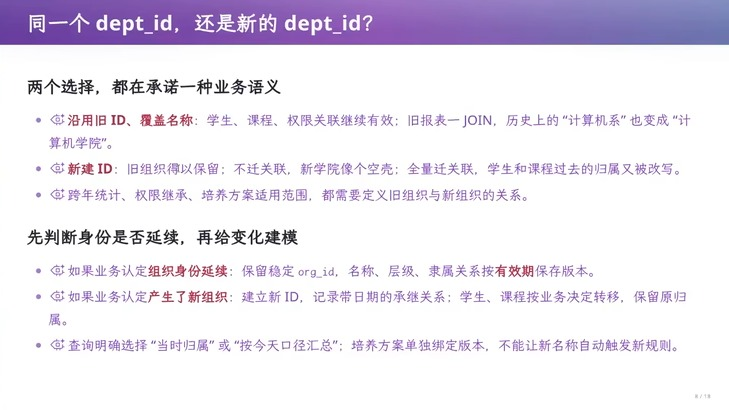
\includegraphics[width=\textwidth]{figures/fig_35_dept_id.jpg}
\caption{同一个 \texttt{dept\_id}，还是新的 \texttt{dept\_id}？两个选择都在承诺一种业务语义；应先判断组织身份是否延续，再给变化建模\vtag}
\end{figure}
\srcnote{01:25:15--01:25:29}

\begin{table}[H]
\centering
\small
\begin{tabular}{p{2.6cm}p{5.4cm}p{5.6cm}}
\toprule
选择 & 带来什么 & 代价 \\
\midrule
沿用旧 ID、覆盖名称 & 学生、课程、权限关联继续有效 & 旧报表一 JOIN，历史上的“计算机系”也变成“计算机学院”；讲者 2011 年的毕业证明会打印成“毕业于计算机学院”，与事实不符 \\
新建 ID & 旧组织得以保留 & 不迁关联，新学院像个空壳；全量迁关联，学生和课程过去的归属又被改写 \\
\bottomrule
\end{tabular}
\caption{院系调整的两种建模选择（据 01:25:15 画面与讲者口述整理）}
\end{table}

幻灯片给出的方向是：先判断身份是否延续，再给变化建模。如果业务认定组织身份延续，就保留稳定的 \texttt{org\_id}，把名称、层级、隶属关系按有效期保存版本；如果认定产生了新组织，就建立新 ID，记录带日期的承继关系，学生、课程按业务决定转移并保留原归属；查询时明确选择“当时归属”还是“按今天口径汇总”，培养方案单独绑定版本，不能让新名称自动触发新规则。

讲者的总结是：如果假设这个世界的投影不变，CRUD 是完美的架构；但只要假设需求会发生摧毁性的变化，每次变化都意味着一次数据库迁移和业务逻辑重写。

\subsection{系统一旦跑起来，修改的代价极高}

\begin{figure}[H]
\centering

\includegraphics[width=\textwidth]{figures/fig_36_migration_cost.jpg}
\caption{系统一旦跑起来，修改的代价极高：代码可以重写，历史不能凭空补出来；同样一个“已毕业”，可能来自正常审核、人工特批，也可能只是某次救火；软件的设计、实现、维护都是手艺活，这也是 ERP 类系统的护城河；迁移需要决定哪些历史含义继续成立，没有保存的依据，AI 也推不回来\vtag}
\end{figure}
\srcnote{01:26:30--01:26:44}

讲者解释了迁移为什么让人“手抖”：数据库事务 update 完成后，就从旧状态彻底挪到了新状态，历史消失了。做一次迁移，要考虑历史上所有可能发生的情况，何况库里已经有很多不一致，很难写出迁移规则；在测试环境里迁移一次，和把学校真实的全部数据迁移一次，难度完全不同，迁完之后库可能就坏了——就像他把缺课次数改成 $-1$ 那样。

所以讲者说，到今天为止，教务系统这类 ERP 系统的设计、实现、维护都是手艺活。他对教务系统的调侃也有另一面：一家可能在 2000 年成立的公司，当年唯一的选择就是参考已有的企业架构做一个教务系统，抢占教育市场的第一桶金；做出来就是一个 CRUD 系统，背上技术债之后，要在中国大学几十年的教育改革中“扛下所有”。

\begin{knowledgebox}{讲者的亲历：研究生院系统的结局}
讲者读博时，隔壁软件工程组接了学校研究生院教务系统的订单，金额可能是二三十万，在学生看来不小，在定制化软件里却是小单，因为之后要不停地维护。讲者当时常和做这个项目的室友争论，认为这个典型的 CRUD 架构最后会遇到各种问题。后来研究生大规模扩招，培养类型增多，调整频繁，这些都是做需求设计时始料未及的，系统最终彻底维护不下去，现在统一换成了公司维护的系统。
\end{knowledgebox}

\subsection{本章小结}

CRUD 用一个一致的当前状态描述世界，范式分解又消除了冗余，这在世界不变时是完美的。教务系统的问题在于世界一直在变：当前状态里的很多字段其实是“事实 + 规则 + 决定”压缩后的结论，压缩丢掉了计算过程；于是例外只能靠手改，语义变化只能靠高风险的迁移，历史一旦覆盖就补不回来。讲者由此提出下一节的问题：既然依赖和历史才是麻烦的根源，能不能把它们直接变成系统里的一等公民？
\section{把历史变成一等公民：Event Sourcing 与 CQRS}

本节回答：如果重做教务系统的架构，讲者会怎样从第一性原理出发避开 CRUD 的困境？代价是什么？

\subsection{从持久化数据结构说起}

讲者说，如果要重做教务系统的架构，他首先看到的是“单一事实来源”太危险：一旦出现不一致，你都不知道该怎样把它找出来。接着他会想到数据结构课上一种“非常神奇的东西”：持久化数据结构（persistent data structure），它能保留数据结构的全部历史。

\begin{figure}[H]
\centering
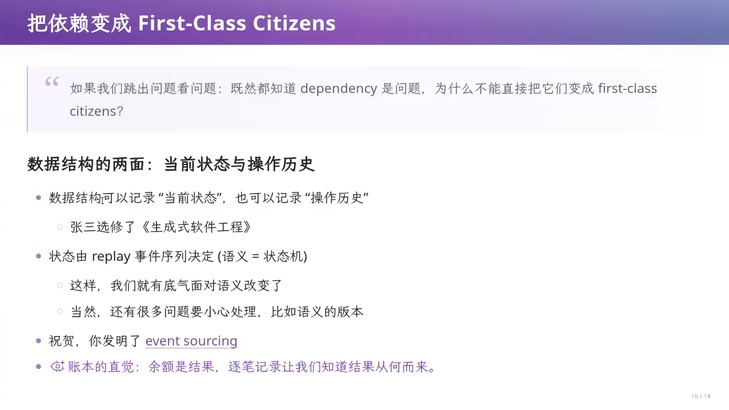
\includegraphics[width=\textwidth]{figures/fig_37_first_class_deps.jpg}\\[4pt]
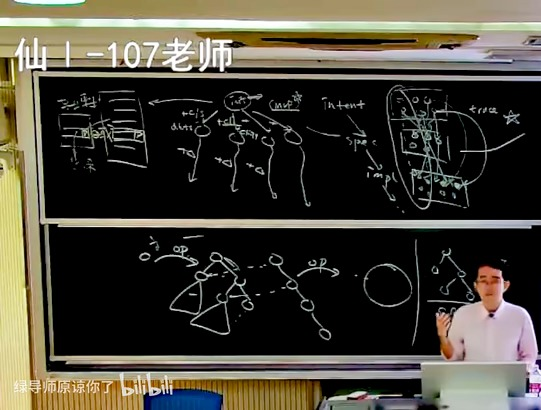
\includegraphics[width=0.72\textwidth]{figures/fig_37_board_history_vs_state.jpg}
\caption{上：把依赖变成 first-class citizens——既然都知道 dependency 是问题，为什么不直接把它们变成一等公民？数据结构可以记录“当前状态”，也可以记录“操作历史”；状态由 replay 事件序列决定。下：板书，左侧是经过一次次操作（op）产生新版本、共享未变部分的持久化树，右侧是只有一个当前状态的 CRUD\vtag}
\end{figure}
\srcnote{01:33:30--01:33:44}

讲者在黑板上对比了两种做法。数据库也是一种数据结构；CRUD 的做法是只存一棵树，对它做一次操作就到下一个状态。持久化的做法是：修改某个节点时，把从它到根的路径复制一份长出来，新的路径指向没变的子树，旧版本仍然完整存在；无论树多大，都存得下。

\begin{importantbox}{三种等价的视图}
讲者指出，可以存状态，也可以存操作，也可以存操作对状态造成的 delta，这三种视图是等价的，都能通过回放历史得到当前状态：
\begin{itemize}
  \item 存操作日志，就是数据库课上的预写式日志（write-ahead log）；
  \item 存 delta，就是 Git、SVN 这类版本管理的思想；
  \item 只存当前状态，就是 CRUD。
\end{itemize}
所以想设计更好的架构，最好先把发生过的所有事情都记下来：今天张三退学了，今天张三又复学了。
\end{importantbox}

用状态机的语言写出来，就是幻灯片上“状态由 replay 事件序列决定”这句话：

\[
S_n = \delta\bigl(\cdots\delta(\delta(S_0, e_1), e_2)\cdots, e_n\bigr)
\]

\begin{itemize}
  \item $S_0$：初始状态（例如空的选课表）；
  \item $e_1,\dots,e_n$：按发生顺序记录的事件，如“张三选修了《生成式软件工程》”；
  \item $\delta$：状态迁移函数，即业务语义——给定状态和事件，得到下一个状态；
  \item $S_n$：回放完前 $n$ 个事件后的当前状态。
\end{itemize}

\subsection{退学、复学与院系调整：回放如何带来底气}

讲者用“复学”这个原来没有的操作说明差别。假设系统原本没有复学操作，张三退学就是把他从数据库里抹掉，某些记录随之删掉。现在要加复学，你必须把他和其他部分的关联重新建起来，代价很大。如果系统记录了所有操作，就可以通过 replay 知道张三退学之前的状态。

讲者也提醒：业务逻辑并不会因此减少，复学之前没考虑过，你依然要为它写一段逻辑。变化在于“事实不可篡改”：世界里所有状态都是事实的投影，你就有了底气，不怕出错。做错了可以很快退回过去的某个快照，修好逻辑再重放，而不像 CRUD 迁移那样“手在抖”。

计算机系改学院的问题也相对好解决。在某个时刻发生一个事件叫“院系调整”。查询一个过去的人，就查到他过去的版本：比如一位同学 2007 年入学、2011 年毕业，属于计算机系；计算机系在 2024 年改为计算机学院。你总可以根据当前关心的事实，裁出一段与之相关的历史，再回放得到需要的状态，既能查过去，也能查现在。讲者说，这就是好的架构设计。幻灯片补充了一句“账本的直觉”：余额是结果，逐笔记录让我们知道结果从何而来。

\subsection{Event Sourcing：从事件历史生成状态}

\begin{figure}[H]
\centering
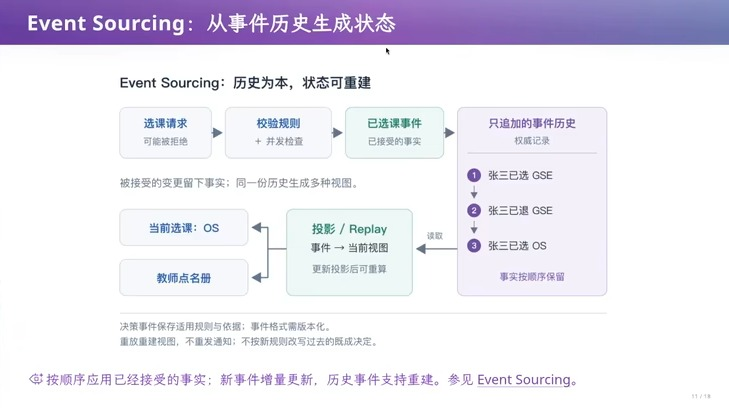
\includegraphics[width=\textwidth]{figures/fig_38_event_sourcing.jpg}
\caption{Event Sourcing：历史为本，状态可重建。选课请求经校验规则与并发检查，被接受后成为“已选课事件”，追加到只追加的事件历史（权威记录）中；投影/Replay 从事件生成当前选课、教师点名册等多种视图。决策事件保存适用规则与依据，事件格式需要版本化；重放只重建视图，不重发通知，也不按新规则改写过去的既成决定\vtag}
\end{figure}
\srcnote{01:35:15--01:35:29}

讲者对听众说：“祝贺你，你就发明了 Event Sourcing。”这是一个经典的设计模式，想法很简单：从历史事件生成状态，而不是直接维护 CRUD 的状态。图中的例子是三条事件：张三已选 GSE、张三已退 GSE、张三已选 OS；回放之后当前选课是 OS。同一份历史可以生成多种视图。

\begin{warningbox}{Event Sourcing 的代价与时机}
讲者预料到的第一个疑问是性能：要大量 replay。他认为这不是大问题，可以用快照、缓存等技巧优化。更实际的限制是时机：如果系统已经是“屎山”，再改成 Event Sourcing 会非常困难；如果从一开始就这样设计，很多问题根本不会发生。幻灯片上的注意事项同样是边界：事件格式要版本化，重放不能重发通知，也不能按新规则改写过去的决定。
\end{warningbox}

讲者还让 Agent 评估：如果用 Event Sourcing 管理那个 AI 生成的教务演示系统，会不会更好？

\begin{figure}[H]
\centering
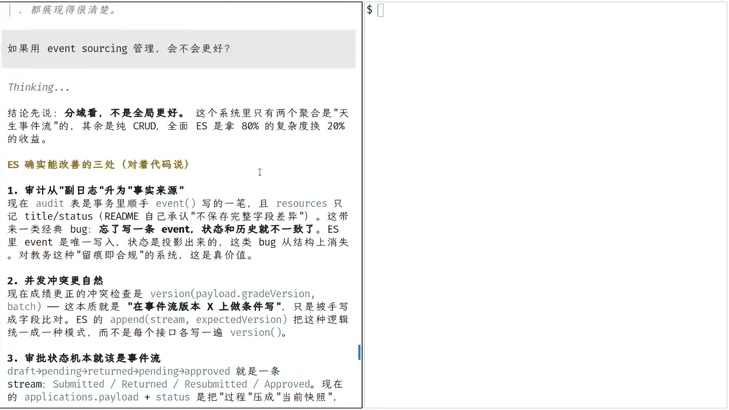
\includegraphics[width=\textwidth]{figures/fig_39_es_tradeoff.jpg}
\caption{Agent 的评估：“结论先说：分域看，不是全局更好。”系统里只有两个聚合是天生的事件流，其余是纯 CRUD；全面 ES 是拿 80\% 的复杂度换 20\% 的收益。ES 确实能改善三处：审计从副日志升为事实来源、并发冲突检查更自然、审批状态机本就是事件流\vtag}
\end{figure}
\srcnote{01:36:00--01:36:14}

\begin{table}[H]
\centering
\small
\begin{tabular}{p{3.0cm}p{10.6cm}}
\toprule
方面 & Agent 的分析（据 01:35:45--01:36:00 画面整理） \\
\midrule
审计 & 现在 audit 是事务里顺手写的一笔，忘写一条 event 就会让状态和历史不一致；ES 里 event 是唯一写入、状态是投影，这类 bug 从结构上消失。对“留痕即合规”的教务系统，这是真价值 \\
并发 & 现在的冲突检查本质是“在事件流版本 X 上做条件写”，ES 的 \texttt{append(stream, expectedVersion)} 把它统一成一种模式 \\
审批 & draft→pending→returned→pending→approved 本就是一条事件流 \\
代价：读模型 & 现在一条大 JOIN 直接出数据；ES 下要维护投影、处理最终一致、考虑重建，系统从“一份状态”变成“两份状态” \\
代价：事件 schema & 业务规则仍在高频演化，事件不可变，规则一变就要写版本化事件和升级器；原型阶段改需求最贵的方式就是 ES \\
\bottomrule
\end{tabular}
\caption{对演示系统采用 Event Sourcing 的收益与代价}
\end{table}

这份评估给讲者的论点加了一个边界：事件历史最有价值的地方，是毕业审核、审批这类“过程本身就是业务”的领域；对纯粹的资料维护，CRUD 依然合适。

\subsection{CQRS：读与写可以有不同的模型}

\begin{figure}[H]
\centering
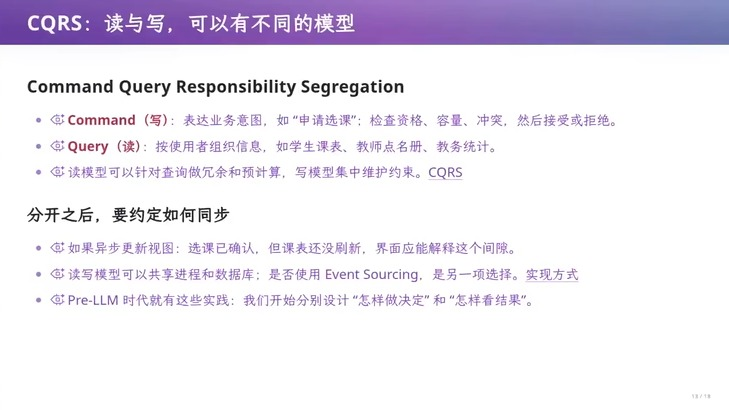
\includegraphics[width=\textwidth]{figures/fig_40_cqrs.jpg}
\caption{CQRS（Command Query Responsibility Segregation）：Command（写）表达业务意图，如“申请选课”，检查资格、容量、冲突后接受或拒绝；Query（读）按使用者组织信息，如学生课表、教师点名册、教务统计；读模型可以为查询做冗余和预计算，写模型集中维护约束。分开之后要约定如何同步，是否使用 Event Sourcing 是另一项选择\vtag}
\end{figure}
\srcnote{01:36:15--01:36:29}

讲者最后提到 CQRS 与 Event Sourcing 是相互独立的两个概念，还有 Domain-Driven Design 之类的“buzzwords”。他的态度是：这些你们都可以去看，但不需要从名词出发。只要回到第一性原理，在设计 50 万行的教务系统时跳出问题，看清它根源上的问题在哪里，哪怕没听说过这些名词，也能做出正确的架构设计。幻灯片补充，这些实践在 LLM 之前就有了：人们开始分别设计“怎样做决定”和“怎样看结果”。

\subsection{本章小结}

CRUD 的困境来自“只保存结论”。Event Sourcing 把事实（事件）当作权威记录，把状态当作可以随时重算的投影，于是例外、语义变化和历史查询都有了表达的位置；CQRS 进一步把“做决定”和“看结果”分成两个模型。代价是投影维护、最终一致和事件版本化，而且最好从一开始就这样设计。讲者用这个例子收束全讲：好的架构不来自记住名词，而来自对需求根源的理解。

\section{总结与延伸}

\subsection{讲者的结论}

讲者在全讲中反复回到两个判断。第一，在 Agentic AI 时代，目标明确的代码已经很便宜，需求、产品设计和架构成了撬动软件生产力的杠杆；不认真对待，它们就会变成 AI Slop 的堆积。第二，架构只有一条方法——跳出问题看问题：10 行的汉诺塔、2000 行的二维码生成器、50 万行的教务系统，都是先看清问题背后的规律，再决定把复杂性放在哪里。

\subsection{本讲义的归纳}

本讲义把全讲压缩为一条链：

\begin{enumerate}
  \item \textbf{需求会变且说不清}，所以每一个已实现的需求都会变成下一个需求的约束（第 3、4 节）。AI 能在一小时内写出一份带编号、可追溯、可验收的需求说明书并实现演示系统，却不能替你预见离散数学拆课、院系调整这类变化。
  \item \textbf{架构的职责是给变化划边界}（第 5 节）。四阶段 \texttt{main}、\texttt{getopt} 的解析状态、二维码的中间语言、事件溯源里的事件日志，都是在易变部分和稳定部分之间插入一个稳定的中间形态。
  \item \textbf{表示的选择决定哪些知识能保留}（第 6、7 节）。汉诺塔的四种写法、Excel 公式与中间语言的对比都说明：同一个需求，换一种表示，难度和对变化的抵抗力都会改变。
  \item \textbf{业务系统的“表示”问题是：保存结论还是保存事实}（第 8、9 节）。CRUD 保存结论，丢掉了事实、规则与决定之间的依赖；Event Sourcing 保存事实，让结论可以重算、可以解释。
\end{enumerate}

\begin{importantbox}{可以带走的检查问题}
\begin{itemize}
  \item 给 AI 下达需求前：这几个字的提示词，会让哪些文件、哪些依赖进入上下文？它们以后好撤回吗？
  \item 设计一个模块时：换一种输入格式、换一个目标平台（如 Excel 版本），需要改到哪里？
  \item 设计一个字段时：它是事实，还是由事实和规则算出来的决定？如果是后者，算它的依据保存在哪里？
  \item 面对一个设计模式名词时：它解决的根源问题是什么？我的系统有没有这个问题？
\end{itemize}
\end{importantbox}

\subsection{边界与下一步}

本讲的论证主要来自一个领域（高校教务系统）和讲者的亲身经历；关于 AI 能力的判断（如“GPT-6 的实现已超越人类理解范畴”“强化学习能引导模型学会抽象机器式的写法”）是讲者基于课堂演示的看法，不是系统评测。Agent 对演示系统的架构评价，也只针对那一个一小时生成的原型。讲者说要用两节课讲需求和架构，本讲是第一部分；下一讲预计会继续讨论架构，讲者也提到会在某次课上专门讲乐观锁、幂等等工程设计。

%% --- 正文内容结束 --- %%

\end{document}
